% Vorlage fuer Thesen an der FFHS
\documentclass{ffhsthesis}

\usepackage[utf8]{inputenc}
\usepackage{parskip}

\usepackage{csquotes}
\usepackage{biblatex}
\addbibresource{references/references.bib}

\usepackage{lipsum}% MWE only

\usepackage{todonotes}
\usepackage{float}
\usepackage[inkscapeformat=png]{svg}
\usepackage{adjustbox}
\usepackage[cache=false,outputdir=.]{minted}

\begin{document}

\raggedbottom
\interlinepenalty=10000

\dokumentTyp{Disposition Bachelorthesis}
\studiengang{INF}
\title{Exploring the Potential of C\# Source Generators for Improving Runtime Performance}
\subtitle{An Evaluation of Reflection-to-Code Conversion Techniques} % optional
% \titelbild[height=2cm,width=10cm]{...}  % optional
\author{Jorge Paravicini}
% \date{}
\wohnort{Zürich}
%\referent{Name des Referenten\\ Titel\\Unterrichtetes Fach}
\referentin{Dr. Ilir Fetai\\PhD Computer Science\\Enterprise Computing}
\eingereichtBei{Oliver Ittig\\Department of Informatics\\Head of Department} 
\dedication{This thesis is dedicated towards\\\dots}
\maketitle
\begin{zusammenfassung}
In dieser Arbeit wird der Einfluss der Verwendung einer statischen Methode zur Identifikation von Aktionen auf die Leistung von ASP.NET Core-Anwendungen untersucht. Im Fokus steht dabei die Anwendung von C\# Source Generators, um den üblicherweise auf Reflexion basierenden Prozess in einen statischen Prozess umzuwandeln. Die Studie analysiert, inwiefern diese Änderung die Startzeit der Anwendung, den Speicherverbrauch und die Build-Dauer beeinflusst. Die Ergebnisse zeigen, dass der statische Ansatz die Startzeit, vor allem bei grösseren Anwendungen, erheblich beschleunigt. Kleinere Anwendungen profitieren ebenfalls, auch wenn die absolut eingesparte Zeit gering ist. Der Speicherverbrauch während des Starts reduziert sich bei der statischen Methode, allerdings kommt es zu einer Verlängerung der Build-Zeit, insbesondere bei grösseren Anwendungen. Die Resultate unterstreichen die potenziellen Vorteile des statischen Ansatzes in ASP.NET Core-Anwendungen, weisen aber auf einen Kompromiss zwischen einer schnelleren Startzeit und einer längeren Build-Zeit hin. Die Arbeit empfiehlt zukünftige Forschungen, die sich auf die Optimierung dieses Kompromisses konzentrieren und die Auswirkungen auf unterschiedliche Anwendungstypen weiter erforschen.
\end{zusammenfassung}

\begin{abstract}
This thesis explores the impact of static action discovery on the performance of ASP.NET Core applications. It evaluates the use of C\# source generators to convert the action discovery process from a reflection-based mechanism to a static one. The study investigates how this conversion affects the application's startup time, memory use, and build time. The findings show that static action discovery significantly speeds up the startup time, especially in larger applications. Smaller applications also benefit, although the absolute time saved is small. Memory usage during startup is lower with static action discovery, but there's an increase in build times, which is particularly evident for larger applications. The results highlight the potential benefits of static action discovery in ASP.NET Core applications while revealing a trade-off between faster startup and longer build times. The thesis suggests that further research could focus on optimizing this trade-off and exploring the impact on different types of applications.
\end{abstract}
\tableofcontents
\include{chapters/14_abbreviations}

\startThesis % Befehl muss vor dem ersten chapter stehen (Seitennummerierung!)

\chapter{Introduction}

New tools and technologies emerge in the constantly evolving software development landscape, promising to streamline development processes and bolster efficiency. One such recent innovation is C\# source generators, a component of the .NET compiler platform that allows developers to generate source code dynamically at compile time. Source generators can inspect and manipulate the code's syntax tree, facilitating the generation of additional source code compiled alongside the existing one.

Introduced in 2020 with the release of C\# 9.0, source generators were a much-awaited tool, a fresh alternative to traditional code generation techniques, which often proved inflexible and maintenance-intensive. With the advent of source generators, developers now have a new instrument in their arsenal, promising to enhance code quality and simplify the development process.

This bachelor's thesis explores the potential benefits and limitations of utilizing C\# source generators in application development. As a relatively new concept, there is much to be discovered about the effectiveness of source generators and the best practices for their efficient use. The thesis aims to fill this knowledge gap by empirically evaluating the application of C\# source generators for boosting runtime performance.

The motivation for this work stems from two main sources: the increasing demand for high-performing enterprise applications capable of complex data processing and an eagerness to explore and understand new .NET technologies, specifically source generators. This thesis hopes to provide valuable insights and practical knowledge for developers aiming to optimize their .NET applications by examining how source generators can be harnessed to improve application performance.

The primary objective of this research is to examine whether employing C\# source generators can improve the runtime performance of ASP.NET web applications. In the fast-paced business world, balancing performance and development speed is crucial. For instance, reflection, a modern approach that allows a program to introspect its structure and behavior at runtime, significantly enhances development speed. However, this comes at the cost of runtime performance. C\# source generators offer a solution to this issue by generating static that would otherwise use reflection during compilation, thus removing the need for runtime reflection.

The guiding research question for this investigation is:

\begin{enumerate}[label=\textbf{RQ.\arabic*}:, leftmargin=*, labelindent=1em]
    \item "How does using C\# source generators to convert reflective action discovery into static code in ASP.NET Core impact startup performance, memory usage, and build time duration?"
\end{enumerate}

The scope of this research is limited to using C\# source generators for generating static code from reflective code, focusing on effects on runtime, build time performance, and memory usage. The research will not consider other factors like code complexity or other potential source generator uses. Additionally, this study will be limited to C\# applications without considering applications written in different programming languages.

\chapter{Relevant Academic Literature and Research}

Performance optimization is a crucial aspect of computer science, with numerous studies exploring its significance and potential areas of enhancement. This section provides a literature review on topics pivotal to this thesis - code generation and optimization, the impact of reflection on performance, the challenges in ASP.NET Core routing, and the current state of research regarding source generators. This exploration of the existing academic literature will identify gaps in recent research and pave the way for the original contributions of this bachelor's thesis.

\section{Code Generation and Optimization}

Code generation and optimization, being essential areas of research within computer science, have the power to augment system performance, reduce memory usage, and boost overall efficiency.

Early studies in this field primarily focused on compiler optimizations. Aho et al. \cite{Aho2007} offer a thorough study of various optimization techniques employed in modern compilers, such as constant folding, dead code elimination, and loop optimizations. Their work underscores the importance of these methods in enhancing the speed of compiled programs.

As the field has evolved, research has branched out to examine dynamic code generation and optimization. Kistler and Franz \cite{Kistler2003} put forward a system that generates code at load-time and continuously optimizes it at runtime. This approach allows the software to adjust to the exact hardware capabilities during execution, thereby overcoming modularization overheads through global optimization. Furthermore, it enables software to adapt to changing user behavior and incorporate dynamic link libraries at a later stage. While they caution that the cost-benefit ratio of continuous optimization can vary, it can lead to speed-ups of more than 120\% under ideal conditions. This indicates the potential of dynamic code generation and optimization when applied correctly.

Recently, machine learning has started to play a significant role in compiler optimization. Madhav, Singaravel, and Karmel \cite{Shreyas2021} discuss how compiler optimization techniques contribute to efficient computing by enabling developers to maximize hardware performance without significant cost implications. Of particular interest in their study is the prospect of machine learning revolutionizing compiler optimization, leading to a more sustainable and efficient computing experience for both developers and users.

The trajectory of code generation and optimization, from early compiler optimizations to recent advancements involving machine learning, demonstrates the ongoing efforts within the software engineering field to elevate software performance. Even as the techniques have evolved, the objective remains consistent - to create efficient, performant, and adaptable software. This historical context underscores the importance of our thesis, which tackles a modern instance of this enduring challenge. By examining the applications and implications of source generators in C\#, we contribute to this ongoing effort to shape and improve software performance. This endeavor remains as relevant today as it was in the early days of software engineering.

\section{Reflection Usage and Performance Implications}

Reflection is a mechanism that allows programs to inspect and manipulate their structure and behavior at runtime. While this capability can be highly beneficial, it also carries performance considerations.

Reflection operations necessitate the dynamic resolution of types, which requires the Common Language Runtime (CLR) in .NET (or equivalent in other languages) to load classes and information at runtime \cite{Tudose2013}. This contrasts with non-reflective code, which loads classes and info at compile time. As a result, reflective operations tend to have slower performance than non-reflective ones due to the additional overhead required for dynamic resolution. An extensive study by Tudose et al. \cite{Tudose2013} states that reflective operations are time-consuming, and developers should avoid frequently calling them if possible due to their performance overhead.

Despite these performance considerations, reflection remains a powerful technique widely used across various programming ecosystems due to its flexibility and adaptability. Specifically, in the .NET ecosystem, an investigation revealed that over 15\% of more than 6 million NuGets utilize reflective techniques \cite{Beaumont2022}. This widespread usage underscores reflection's inherent value and versatility in software development, even in the face of potential performance costs.

This dichotomy—reflection's widespread use and the associated performance penalties—highlights the necessity for alternative strategies. Pursuing mechanisms that provide reflection-like flexibility with more optimal performance characteristics is gaining importance.

The study \cite{Beaumont2022} emphasizes that understanding and employing reflection techniques are valuable for developers at all stages of their careers, yet also cautions about potential performance implications. This reality underscores the need for performant alternatives to support the significant portion of NuGets relying on reflection, potentially enhancing their performance while retaining their functionality.

\section{Performance Implications of ASP.NET Core Routing}

ASP.NET Core is a renowned technology for building web applications and APIs. Its appeal among developers is primarily influenced by its performance attributes - execution speed, delivery time, and startup time.

A comparison study by Kronis and Uhanova \cite{Kronis2018} delved into the performance characteristics of ASP.NET Core and Java EE. They created benchmarks as REST services that processed data in JSON format and ran these benchmarks on the Kestrel web server. Although their investigation did not directly address startup time, it provided valuable insights into the relative performance capabilities of these two platforms.

Karlsson \cite{Karlsson2021} took a slightly different approach, pitting ASP.NET Core and Express.js against each other, using both alongside a MySQL database to construct Web APIs. Karlsson's findings revealed that, in the context of a RESTful API, ASP.NET Core handled lower loads more efficiently, but Express.js had the upper hand when processing a larger volume of concurrent requests. Interestingly, with the new querying language GraphQL, Express.js either equaled or surpassed ASP.NET Core regarding response times and resource usage.

The action discovery process in ASP.NET Core, which utilizes reflection to associate actions with controller routes, might represent a potential performance bottleneck due to the well-known overheads linked with reflection \cite{Beaumont2022}. However, despite the importance of this process, it has been largely overlooked in research, leading to a lack of comprehensive understanding of its effects on application startup time and performance. Therefore, a more thorough investigation of this process is needed. Exploring ways to refine it, mainly to reduce its reliance on reflection, could lead to significant enhancements in startup times of ASP.NET Core applications, underlining the need for an empirical study.

\section{Source Generators and Performance Improvements}

In the relatively uncharted domain of source generators in C\#, Slimak's work \cite{Slimak2022} stands out. His thesis offers an in-depth guide to source generators. The thesis aims to help readers understand source generators, their purpose and use cases, and how they differentiate from other prevalent code generation options in C\#. The work further explores the use of source generators in enterprise applications and proposes a more complex framework that could generate standard boilerplate code, thus improving development efficiency. However, the thesis underscores source generators' current immaturity and challenges for integration into existing .NET tools, like Visual Studio and IntelliSense.

Supplementing the insights from Slimak's research, another study worth discussing is Franz's \cite{Franz2022}, entitled "Trends im Compilerbau." Though written in German, the paper provides a broader view of the trends shaping the field of compiler construction, with a particular focus on source generators and Just-In-Time Compilers. Using a dataset from the IEEE Xplore library, Franz emphasizes how active and vibrant the compiler construction research field remains, even with its considerable history. The emergence of new tools, like source generators, is sparking fresh inquiries. A key takeaway from Franz's study is the sustained focus on code optimizations. These efforts to enhance the output performance of compilers remain a primary concern in both practical and research contexts.

Adding to these scholarly resources, the book "Introducing .NET 6" by Nico Vermeir \cite{Vermeir2022} offers a practical perspective. Though not a research paper, the book contains a chapter titled ".NET Compiler Platform" that explains source generators, among other topics. Vermeir describes how the .NET Compiler Platform, previously known as Project Roslyn, provides strength and flexibility to .NET. Additionally, the author discusses source generators, highlighting how they leverage Roslyn to generate code at compile time and incorporate that generated code into the compilation process.

\section{Strengths, Weaknesses, and Gaps in the Existing Research}

The existing body of literature presents a wealth of information, with various studies investigating different aspects of code generation and optimization. This comprehensive coverage, spanning from early compiler optimizations \cite{Aho2007} to dynamic code generation techniques \cite{Kistler2003}, and even to the incorporation of machine learning \cite{Shreyas2021}, offers a solid foundation for understanding the significance of software optimization. Additionally, the studies delve into the performance implications of reflection and its extensive usage despite the associated overhead \cite{Tudose2013, Beaumont2022}.

Simultaneously, focused examinations such as Slimak's thesis \cite{Slimak2022} and Franz's paper \cite{Franz2022} shine a light on practical applications of source generators and ongoing trends in compiler construction. The literature also includes a comparative performance analysis of ASP.NET Core against other frameworks \cite{Kronis2018, Karlsson2021}, further enriching our understanding of this field.

However, specific gaps and limitations persist in the current research landscape. While the intersection of machine learning and compiler optimization is broached \cite{Shreyas2021}, there's room for a deeper exploration. Moreover, despite acknowledging the reflection's performance cost, alternatives that retain its flexibility without compromising performance remain underexplored.

Significantly, the startup phase of ASP.NET Core applications, potentially impacted by action discovery and routing mechanism performance, has received limited attention. While comparative studies shed light on ASP.NET Core's request handling capabilities, more granular studies focused on its startup phase, particularly the action discovery process, are noticeably absent.

There's also a noted inconsistency regarding the efficacy of continuous optimization for dynamic code generation \cite{Kistler2003}, suggesting a need for more research to discern the specific conditions that maximize these techniques' benefits. Lastly, the immaturity of source generators and their integration challenges with existing .NET tools, as highlighted by Slimak \cite{Slimak2022}, underscores the need for more dedicated research.

\section{Contribution of this thesis}

This thesis contributes to the current body of knowledge in several ways, bridging existing gaps and enhancing our understanding of critical issues about code generation, optimization, and performance improvement in software development.

Firstly, this research expands on the application of source generators in the .NET ecosystem, primarily focusing on performance optimization. Despite the promising potential of source generators, previous research indicates that this technology is currently in a state of relative immaturity \cite{Slimak2022}. This thesis contributes a systematic analysis of source generators, evaluating their strengths, weaknesses, and application areas in the context of software performance improvement.

Secondly, this thesis critically investigates the impact of ASP.NET Core's routing mechanisms on performance—a subject that has received limited attention in the existing literature. By thoroughly examining routing mechanisms and their relationship to startup time, the study uncovers new ways to enhance the performance of ASP.NET Core applications.

Lastly, concerning reflection, existing research has highlighted its associated performance overhead. This study delves into a practical approach to alleviate these performance implications without forsaking the benefits of reflection. Rather than seeking alternatives to reflection, the study attempts to reduce the need for reflection at runtime, thereby preserving its functionality and versatility.
\chapter{Methods for Design, Implementation, and Performance Evaluation of Static Action Discovery}

This section outlines the methods and materials used to create, benchmark, and assess a new action discovery. Initially, we discuss the benchmark application that employs Microsoft's existing dynamic action discovery, serving as the basis for our study. Subsequently, we explore the modified application, highlighting its differences from the benchmark. The implementation details will be further addressed in the next chapter. Lastly, we define the testing metrics, scenarios, and environments used and explain how we ensured the reproducibility of our results.


\section{Characteristics of the Benchmark Application}

This subsection delves into the specifics of the \href{https://github.com/jorgeparavicini/aspnetcore/tree/feature/static-mvc/src/Mvc/samples}{benchmark application} \footnote{\url{https://github.com/jorgeparavicini/aspnetcore/tree/feature/static-mvc/src/Mvc/samples}} used in this research, developed as an ASP.NET Core Web API. A key characteristic of this application, and indeed a cornerstone of its design, is the usage of reflection-based routing discovery. While widely employed, this mechanism inspects every class within the project and loaded assemblies. As the codebase grows, the efficiency of this approach decreases, presenting a challenge that our new implementation seeks to overcome.

The benchmark application is constructed with simplicity in mind, serving as a baseline for evaluating our novel routing implementation. Yet, despite its simplicity, it effectively mimics a small, medium, and enterprise application. We do this by varying the number of controllers present. Each controller varies in complexity, each with a different number of exposed actions and diverse routing attributes. This setup simulates scenarios commonly encountered in a real-world Web API.

A point of significance is that the benchmark application, like our modified app, is written as part of the official ASP.NET Core repository. Our implementation requirements motivate this choice, which involves modifying the existing framework and adding new features. Such changes couldn't have been achieved through an external NuGet package. We've ensured a consistent environment for both apps to provide the most accurate comparisons, thus minimizing potential interference from variables like differing .NET SDKs, hardware, or application setup.

The benchmark application is kept simple, focusing on the core functionalities of a Web API to maximize testing accuracy. By excluding additional features such as authentication or Cross-Origin Resource Sharing (CORS), we eliminate the potential overhead that would equally affect both the standard and modified applications, thereby enhancing the precision of our tests.

Lastly, we've designed the benchmark setup with a focus on reproducibility. The comprehensive description of the application's structure and configurations in this section offers a path for others to replicate these tests and reproduce our results. This ensures that the results we gather are not biased due to extraneous variables, thereby improving the repeatability and reliability of our tests.

\section{Enhancing Action Discovery: A New Perspective}

As we explore static action discovery, we'll see how it restructures traditional applications. The sections below delve into this transformative process, highlighting its impact on routing. We then introduce the concept of static action discovery, providing a comprehensive view of its development. By journeying through these stages, we aim to provide a solid understanding of this new structure and its potential performance benefits.

\subsection{Understanding Action Discovery and Its Role in Routing}

ASP.NET Core is a web framework designed to process various user requests. Based on incoming URLs, HTTP Methods, and Bodies, these requests are directed toward specific actions. Actions can be routed in two distinct ways: via conventional routes, manually defined during the start-up phase, or via attribute-based routing, where routes are defined through annotations on the controllers and their actions.

Figure \ref{fig:conventional-routing} depicts a conventional routing approach. In this example, a route named \texttt{default} is created, generating a pattern against which routes are matched. The route path is tokenized into controllers, actions, and parameters. The extracted tokens correspond to the components of an application. However, manually declaring all routes is time-consuming and error-prone, as routes must always be synchronized with the controllers.

\begin{figure}[H]
\centering
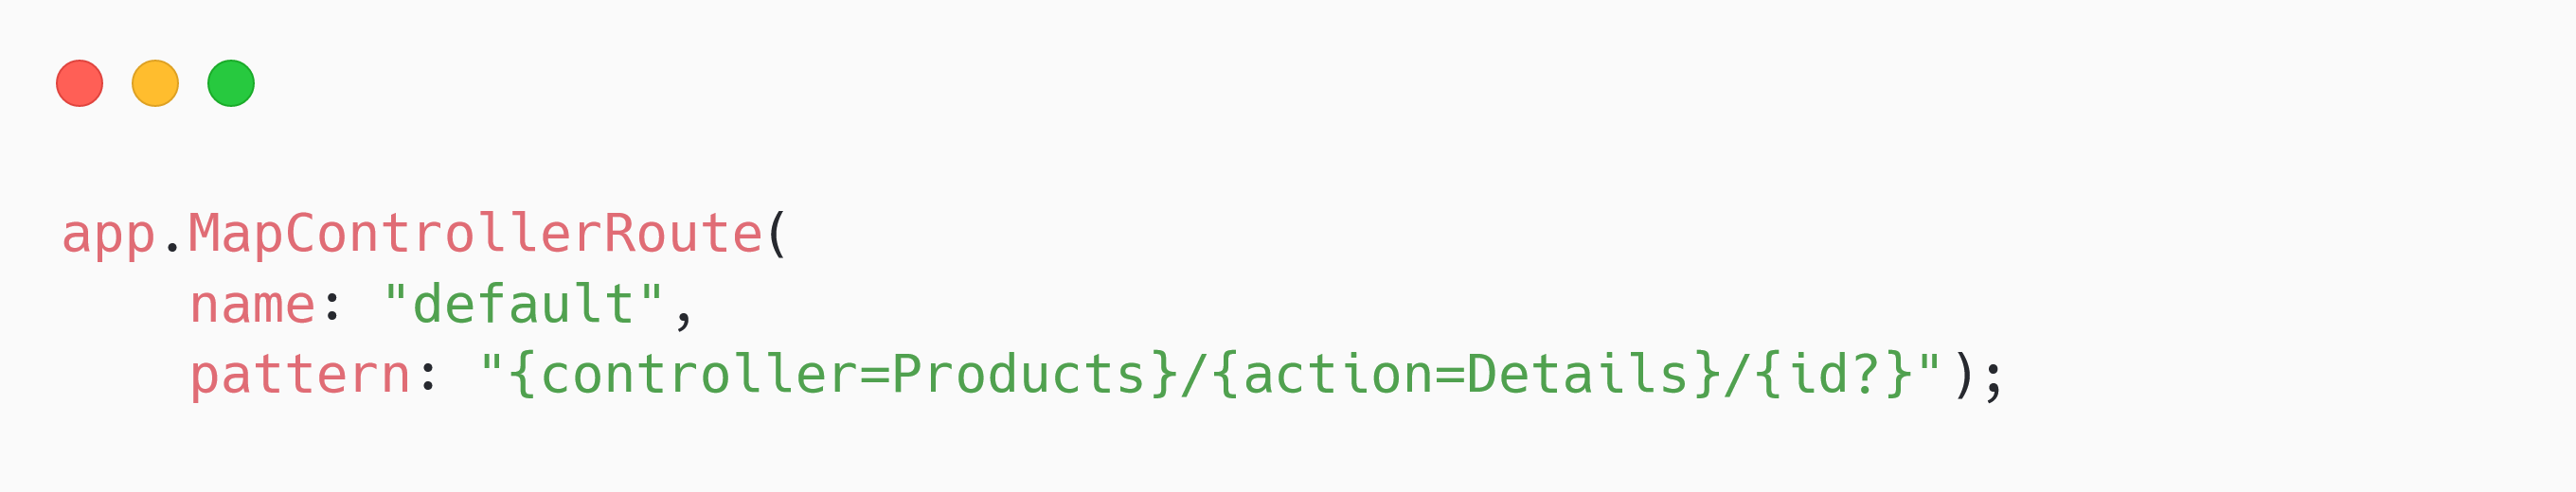
\includegraphics[width=0.8\textwidth]{graphics/conventional-routing.png}
\caption{An example of conventional routing in ASP.NET Core}
\label{fig:conventional-routing}
\end{figure}

To overcome the limitations of conventional routing, attribute-based routing is often used. Here, routes are declared on the controllers directly via attributes, ensuring synchronization between the routes and the controllers and eliminating manual intervention. Figure \ref{fig:attribute-routing} showcases a similar controller as depicted in Figure \ref{fig:conventional-routing}, but with attribute-based routing.

\begin{figure}[H]
\centering
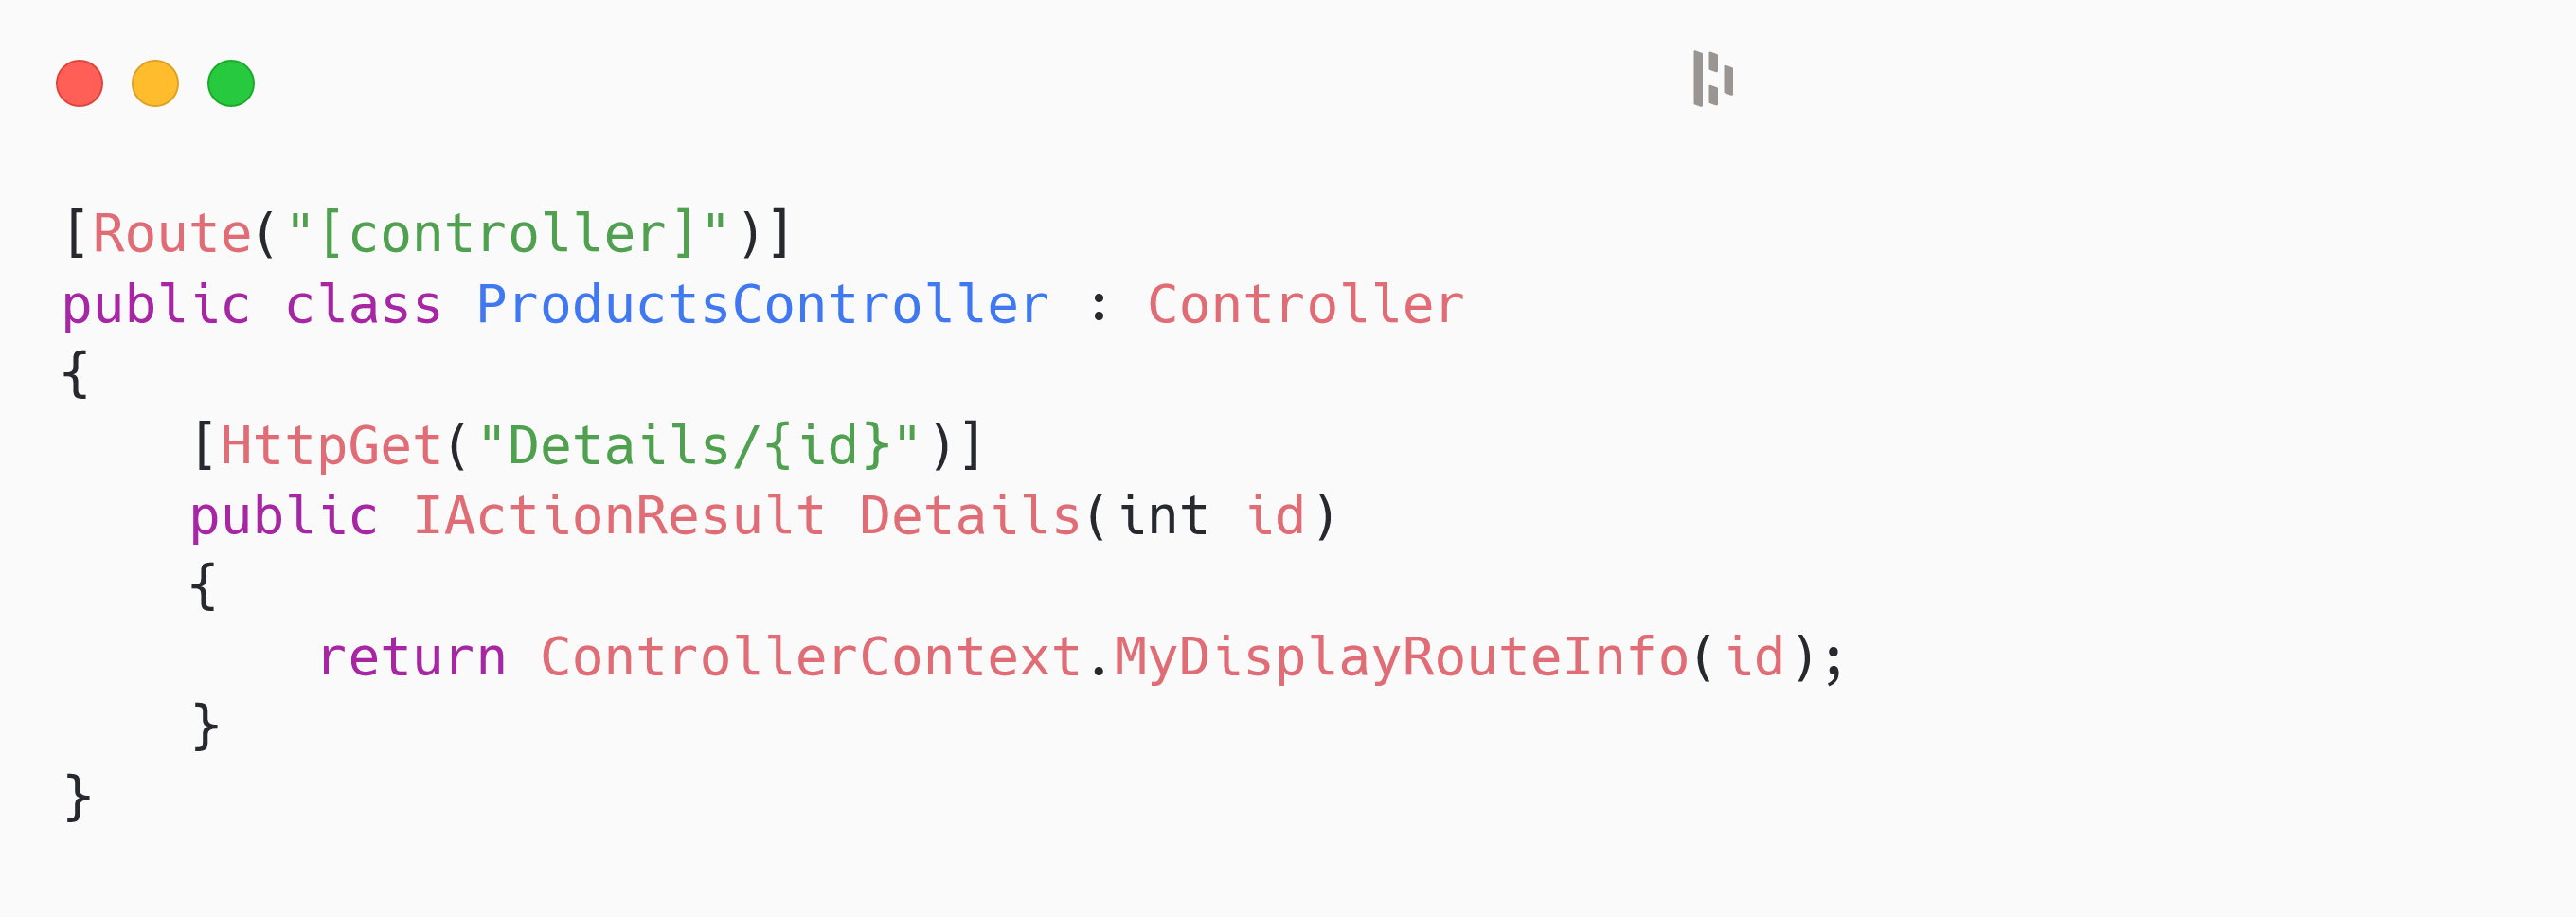
\includegraphics[width=0.8\textwidth]{graphics/attribute-routing.png}
\caption{An example of attribute-based routing in ASP.NET Core}
\label{fig:attribute-routing}
\end{figure}

While attribute-based routing offers an improvement over conventional routing, both approaches have a common drawback: the routing mechanism requires a thorough knowledge of all controllers and actions. Therefore, during the application's start-up phase, a process known as 'action discovery' is initiated, which examines the entire code base to identify all controllers and their corresponding actions.

During application start-up, this action discovery process is launched by calling the \texttt{app.Map\\Controllers()} method. The action discovery involves two significant services registered by the MVC framework. The first service analyzes every file in all referenced assemblies, including third-party tools like Swagger, identifying potential controllers. These identified controllers are then analyzed by a second service, which uses reflection to extract all the routing information.

Although this process is thorough, it can be resource-intensive for larger applications, resulting in performance overhead each time the application is started. Our new tool aims to mitigate this overhead by generating static code at compile time without reflection, optimizing the action discovery process. This tool and its workings will be discussed in detail in the next section.

\subsection{Introducing the Static Action Discovery}

In our approach, we rely on incremental source generators. These tools come into play during the application's build process, producing additional source code that becomes part of the final executable. Crucially, source generators are designed for efficiency, executing only when a change in the output is detected. The nitty-gritty details of this process will be delved into in Appendix \ref{appendix:implementation}, which is devoted to the implementation details.

Our \href{https://github.com/jorgeparavicini/aspnetcore/tree/feature/static-mvc/src/Mvc/Mvc.Generators/src}{source generator} \footnote{\url{https://github.com/jorgeparavicini/aspnetcore/tree/feature/static-mvc/src/Mvc/Mvc.Generators/src}}, during its operation, creates several key files. It spawns a service extension, which allows adding the required MVC framework without needing dynamic action discovery. Furthermore, a unique static action discovery service is created for every controller found within the project.

Let's compare this to the conventional way of integrating the MVC framework into an ASP.NET Core application. This process is illustrated in Figure \ref{fig:dynamic-action-discovery}.

\begin{figure}[H]
\centering
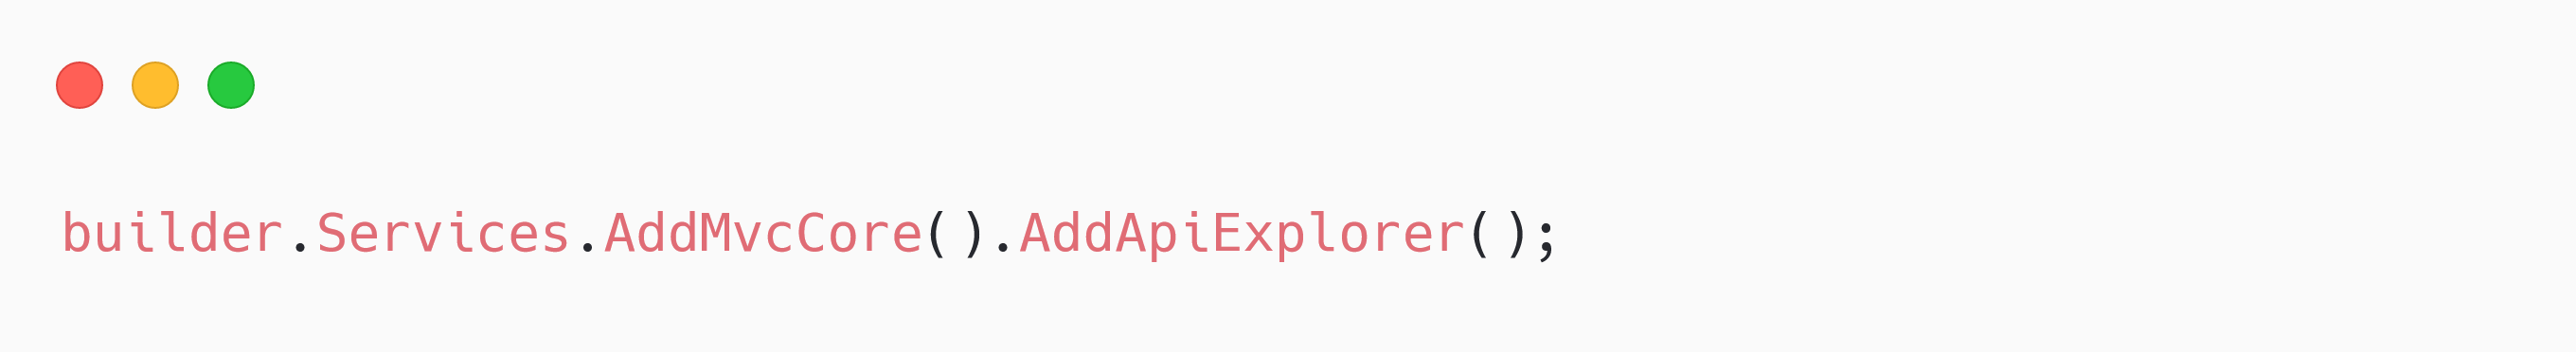
\includegraphics[width=0.8\textwidth]{graphics/dynamic-action-discovery.png}
\caption{Adding the MVC Framework in a traditional ASP.NET Core Application}
\label{fig:dynamic-action-discovery}
\end{figure}

Moving on to our proposed approach, we keep the registration as similar as possible, as shown in Figure \ref{fig:static-action-discovery}.

\begin{figure}[H]
\centering
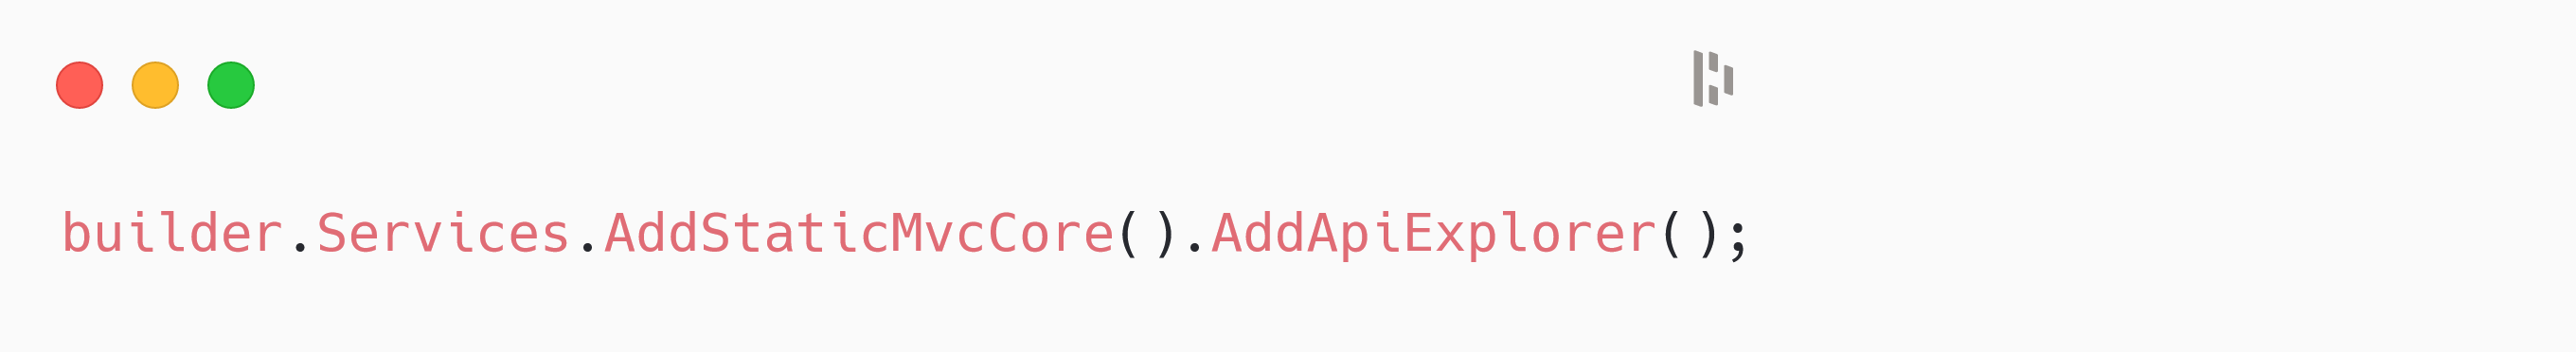
\includegraphics[width=0.8\textwidth]{graphics/static-action-discovery.png}
\caption{Adding the MVC Framework using our new approach}
\label{fig:static-action-discovery}
\end{figure}

While the methods appear virtually identical, it's worth noting that the \texttt{AddStaticMvcCore} method is neither stored in any Git repository nor is it part of the project where the source generator is defined. Instead, it is generated by the project that consumes the source generator, allowing the method to be custom-tailored to each application for potential action discovery optimization.

The \texttt{AddStaticMvcCore} method registers the MVC framework and an action discovery service for every controller in the project under development. The services contain all metadata the routing mechanism requires to map endpoints to the controllers.

A significant challenge arises due to source generators running as part of the compilation process, making reflection an impractical tool. Reflection, used in dynamic action discovery, inspects controllers and reads all the attributes applied to the controllers and actions. However, reflection is unusable since the code is not compiled and cannot be run yet. Instead, we use the Roslyn API to inspect the Syntax Tree and the Semantic Model of the controllers.

The Syntax Tree and Semantic Model allow us to extract the necessary information in a manner similar to reflection but without running the code. However, this means we can only extract information that can be parsed deterministically at compile time, excluding the values of properties or execution of code snippets.

Fortunately, the static action discovery relies on Attributes, the parameters of which must be compile-time constants and can be evaluated. The challenge arises when these attributes use properties that don't fall under the same restriction. Figure \ref{fig:custom-property} shows an example of such an attribute.

\begin{figure}[H]
\centering
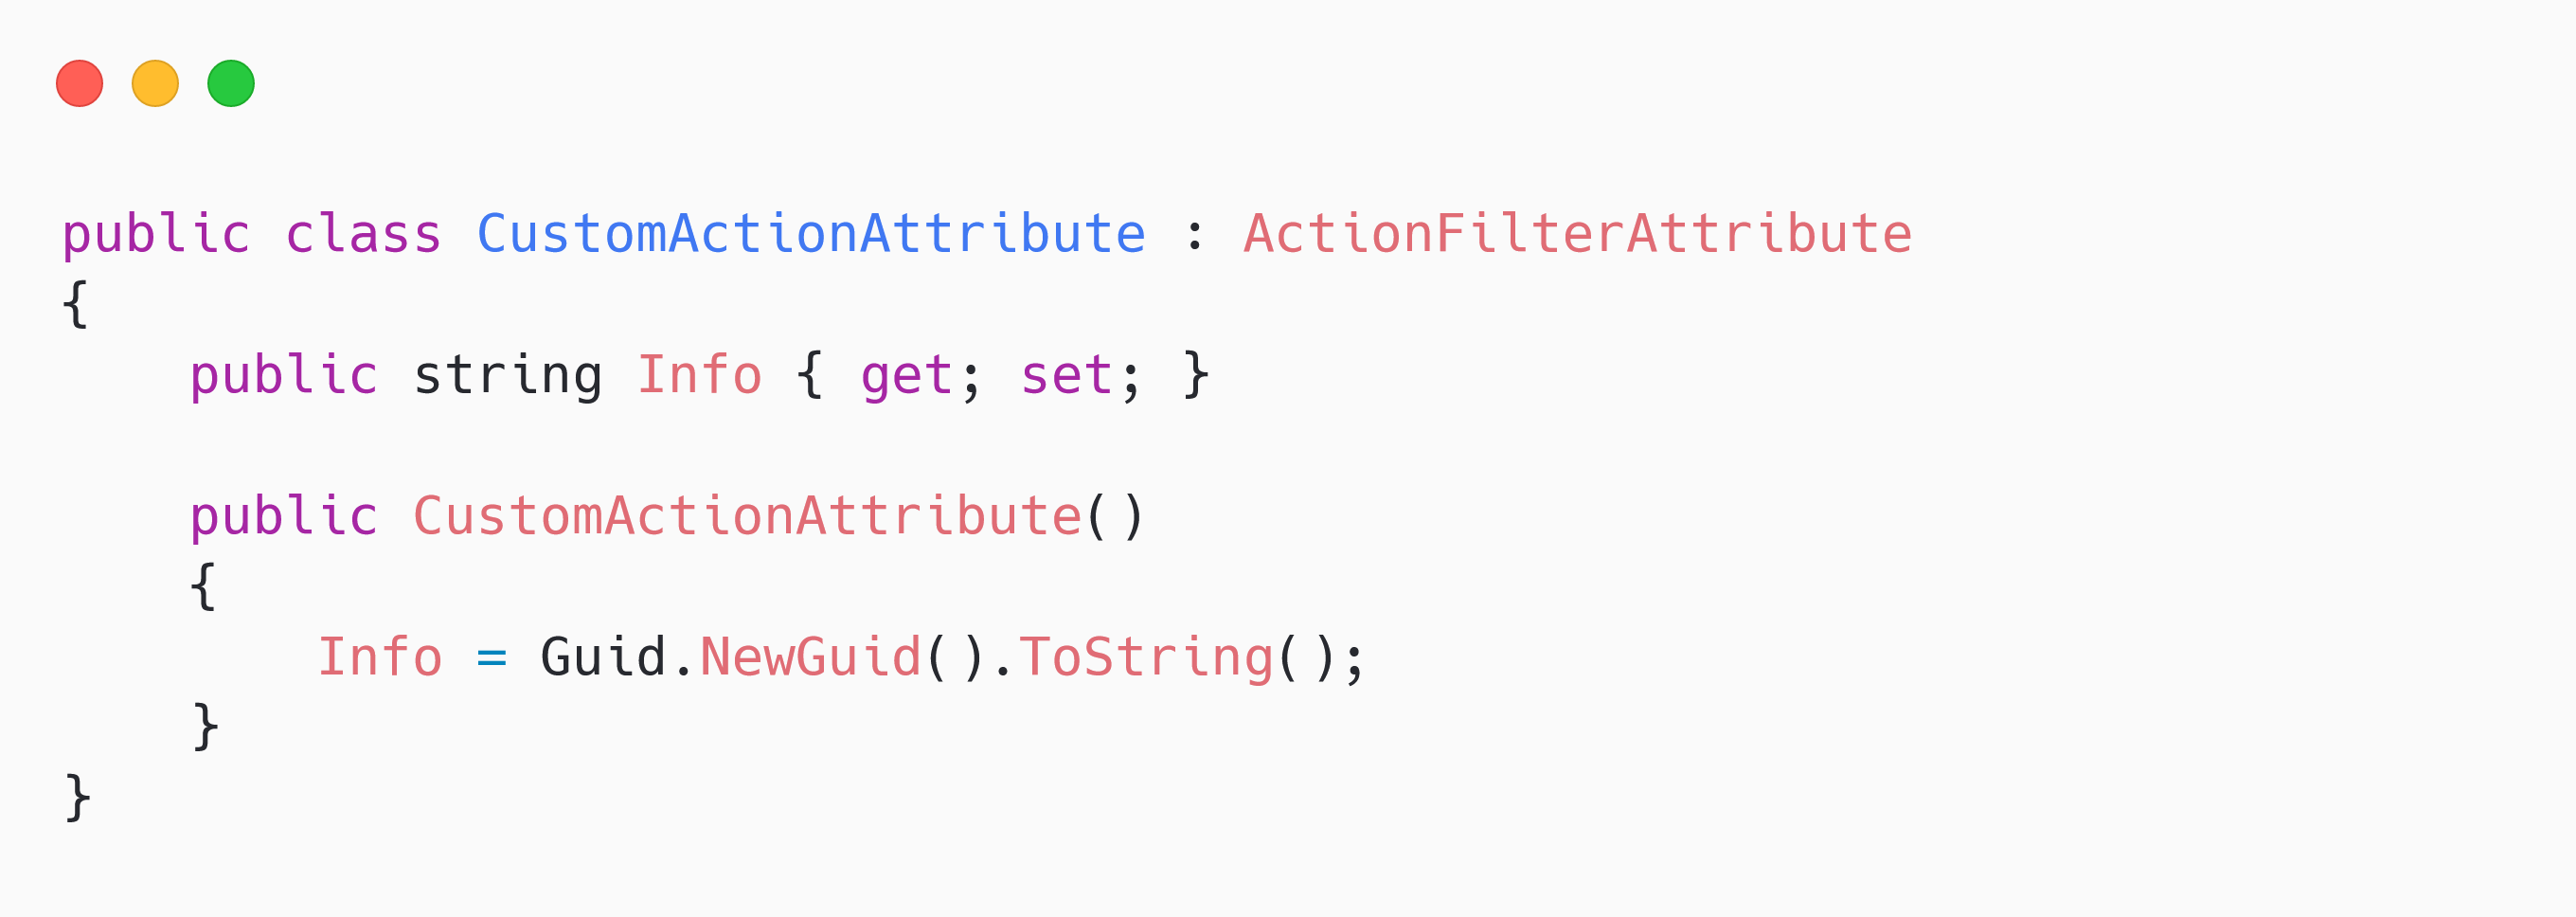
\includegraphics[width=0.8\textwidth]{graphics/custom-property.png}
\caption{Example of a Custom Attribute with Non-deterministic Property Value}
\label{fig:custom-property}
\end{figure}

Upon extracting the required attributes, they are stored as static source code added to the application model executed during the startup. The routing mechanism receives the same application model it would with dynamic action discovery, ensuring seamless integration.

\subsection{Project Structure Options and Decisions}

Two primary strategies emerge when developing a source generator for static action discovery: creating a standalone repository referencing the ASP.NET Core SDK or modifying the official ASP.NET Core repository directly. Each of these approaches carries its own set of advantages and disadvantages.

Creating a new repository provides the advantage of an easy and straightforward setup process. However, it brings along a significant drawback. It doesn't allow for modifying the existing implementation of the MVC framework, which is crucial for our project. The need to remove the dynamic action discovery services implies that after registering the MVC framework, one would have to loop over all registered services in the Dependency Injection container and discard those related to dynamic action discovery. This approach is far from clean, incurs an avoidable performance overhead, and contradicts our project's main goal - minimizing performance overhead. Leaving the dynamic action discovery services as they are would lead to both static and dynamic action discoveries running simultaneously. This would undeniably increase the startup time and potentially cause parts of the application to malfunction due to the ambiguity of endpoints, created twice in this scenario.

In contrast, modifying the official ASP.NET Core repository provides a more elegant solution. It allows for the MVC framework's modification to exclude dynamic action discovery when static action discovery is in use. Importantly, it enables us to include the generators as part of the SDK, enhancing the end user's ease of use. The only requirement for utilizing the generated static action discovery is referencing the generator project, informing the compiler about its existence, and triggering the generation process during builds, where the latter two points happen automatically.

In addition to these points, using the official repository has a few more benefits. It provides direct access to ASP.NET Core's latest updates and features. Also, modifications made in the official repository contribute directly to the ASP.NET Core community, enhancing the open-source ecosystem's vitality and productivity.

\subsection{Approaches to Static Code Generation}

Once the overarching project structure has been settled, the next step is creating the static code representing the application model. For this task, we have two viable options at our disposal: building a string representation of the source code or employing SyntaxFactory.

String representation, although straightforward, tends to be error-prone and challenging to maintain. On the other hand, SyntaxFactory, while verbose and having a slight overhead, offers a more reliable approach. It facilitates creating individual statements, allows easy renaming of variables, and ensures that the resulting source code is syntactically correct and automatically formatted. Despite its overhead, the numerous benefits provided by SyntaxFactory greatly outweigh its drawbacks, making it our preferred choice for this task. 

Figure \ref{fig:syntax-factory} depicts an example of SyntaxFactory's utilization. It demonstrates creating a simple method, accepting a string parameter, and returning a new ControllerModel. It's important to note that the actual method body isn't included within this segment and will be integrated into subsequent portions of the code. This example illustrates the flexibility offered by SyntaxFactory, enabling us to modularize the code generation process effectively.

\begin{figure}[H]
\centering
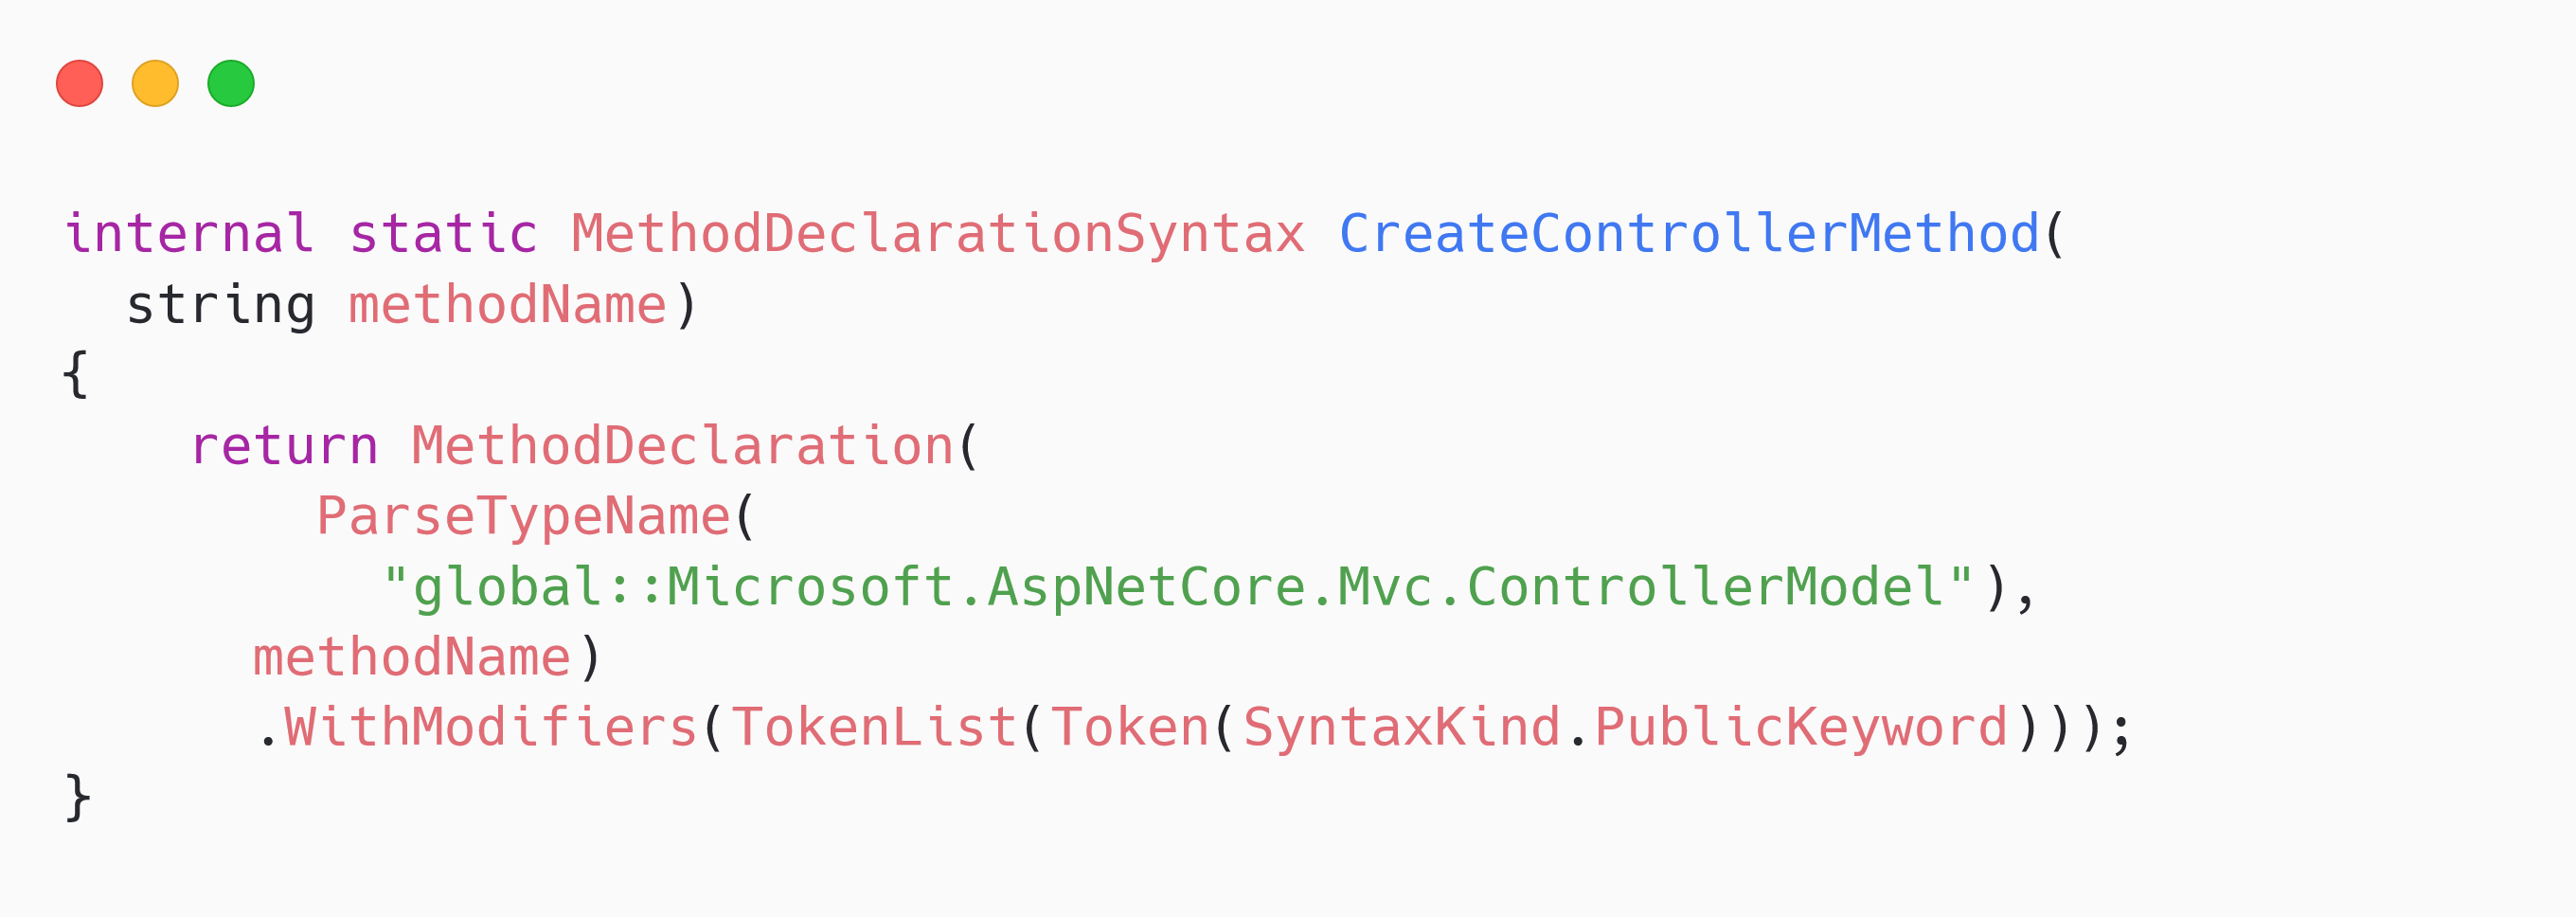
\includegraphics[width=0.8\textwidth]{graphics/syntax-factory.png}
\caption{An example of using SyntaxFactory to generate source code}
\label{fig:syntax-factory}
\end{figure}

\section{Performance Metrics and Evaluation}

To answer our research question— "How does using C\# source generators to convert reflective action discovery into static code in ASP.NET Core impact startup performance, memory usage, and build time duration?"—we need an accurate way of benchmarking the dynamic and static action discovery test applications. The ultimate goal is to determine if static action discovery is a viable approach to reduce the startup time of ASP.NET Core applications and understand the impact of static action discovery on build time and memory usage.

\subsection{Choice of Metrics}

In our quest to determine the impact of using C\# source generators to convert reflective routing operations into static code in ASP.NET Core, three pivotal metrics were chosen—startup duration, build time, and memory usage during startup. The selection of these metrics was driven by enhancing operational efficiency in enterprise environments, particularly in cloud deployments.

The speed at which an application starts up is paramount in contexts like serverless architectures, where applications are frequently spun up and shut down. Consequently, startup duration was selected as one of our primary metrics. An expedited startup process could notably decrease operational costs and foster scalability, two objectives that are crucial for enterprise companies striving to improve their workflows.

Our second metric, build time, was chosen to ensure that the introduction of static action discovery does not excessively impede developer productivity. Lengthy build times could potentially slow down the development process, posing challenges, especially in agile development environments that rely on rapid iteration cycles. Moreover, in the context of continuous integration / continuous deployment (CI/CD) scenarios, long build times could delay the deployment of updates and fixes, adversely affecting the flexibility and velocity of a team's development operations.

Lastly, we chose to monitor memory usage during startup. In real-world systems, memory is a finite and valuable resource integral to application performance. Excessive memory usage can induce a variety of adverse effects. It can worsen the startup process, as the system might need to allocate and deallocate memory. It could also strain the performance of other applications sharing the same system due to the heightened pressure on its memory resources. High memory usage can inflate operational costs in cloud-based environments, where applications are billed based on resource consumption. Moreover, applications that require less memory are generally easier to scale and distribute across various instances.

We also contemplated other metrics, such as Request Handling Time, CPU Usage, and Request Throughput. However, these were ultimately dismissed from our selection as they would remain unaffected by our approach. After the application has started, the produced application model, containing all the information required by the routing mechanism, remains identical whether the dynamic or the static action discovery creates it. The sole difference lies in constructing the application model; its subsequent usage remains constant. Concerning CPU Usage, we concluded that Startup Speed provided a more comprehensive gauge of the startup performance of the two benchmark applications.

\subsection{Benchmarking the Action Discovery}

Defining startup duration requires careful consideration. While the most straightforward approach might be to time the execution of the main function of our application, this approach proves inadequate. Figure \ref{fig:startup-method} shows an example main function.

\begin{figure}[H]
\centering
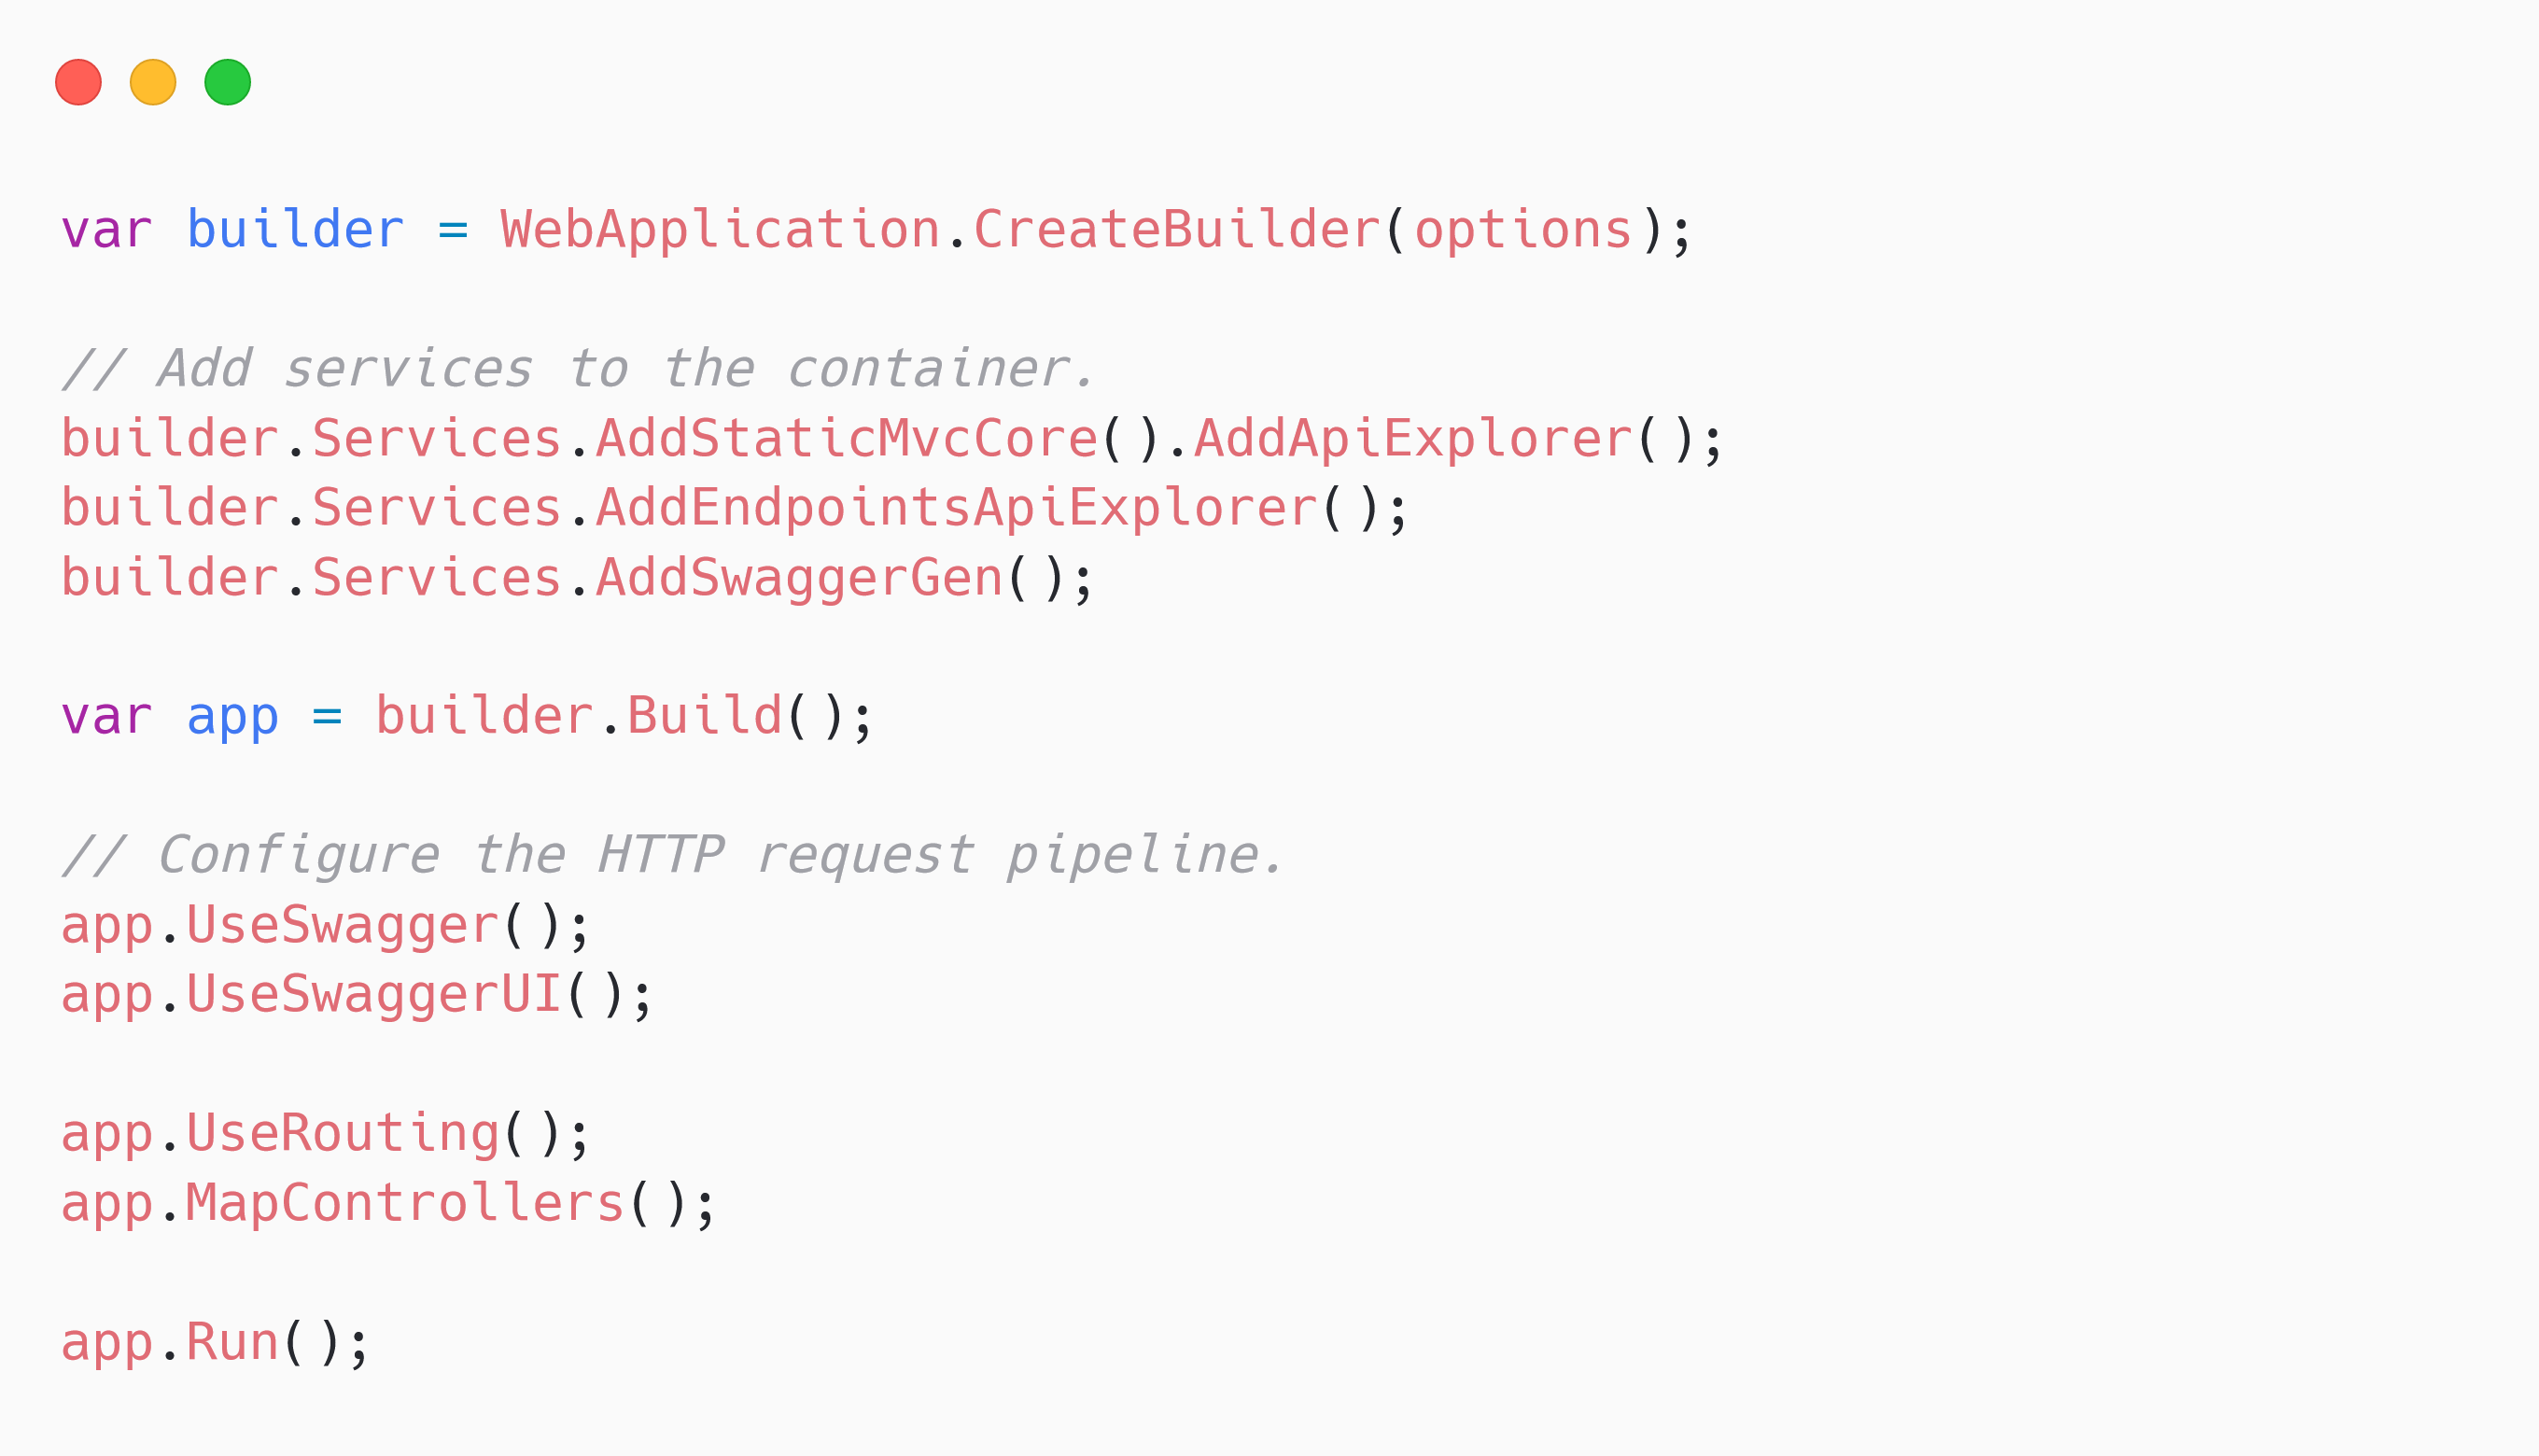
\includegraphics[width=0.8\textwidth]{graphics/startup-method.png}
\caption{The main function of the application, responsible for initializing and running the web server}
\label{fig:startup-method}
\end{figure}

The reason for this lies in the functionality of the \texttt{app.Run()} method in the code, which initiates a loop for the web application that only concludes once the application shuts down.

Another alternative could be to time the execution of the MapControllers() method since it performs the action discovery. However, this method does not accurately represent the total startup time of the application.

To navigate these complications, we capture the "ServerReady" log message, which \texttt{app.Run()} logs when the server is ready to receive user requests. Thus, the startup time is defined as the duration from the start of the main method execution until the "ServerReady" log message is logged.

Regarding the methods for measuring time and memory, the initial thought might be to use a Stopwatch provided by the .NET framework. The Stopwatch would start before the main function execution and stop when the "ServerReady" message is received. However, to ensure the reliability of the results, one would need to execute several warm-up iterations until the benchmark achieves a steady state, perform the main iterations multiple times, and then calculate the necessary statistics.

Given these considerations, it's more efficient to use a dedicated framework. Several frameworks are available in .NET, including BenchmarkDotNet, NBench, MiniProfiler, and Perfolizer. It is based on popularity, as gauged by \href{https://github.com/topics/benchmarking?l=c%23}{GitHub} \footnote{\url{https://github.com/topics/benchmarking?l=c\%23}}), and the fact that Microsoft uses it for benchmarking in the official ASP.NET Core repository, we choose BenchmarkDotNet. Furthermore, BenchmarkDotNet allows us to measure allocated heap memory, which is used to evaluate memory usage during startup.

Finally, measuring build time is executed using the official MSBuild tool, Microsoft's compiler. However, this task is not as simple as it might seem. The project is housed within the official ASP.NET Core repository, which contains over 550 projects. To acquire meaningful results, we compile all dependent projects before measuring the build time and instruct the tool to compile the target benchmark application.

The measurement of build time also needs to be conducted multiple times to ensure the results are meaningful. The build results are cached after every build, which can drastically alter build times after the initial build. Therefore, we ensure that all artifacts related only to the project, not its dependencies, are cleared between builds. As the build time is designed to assess the impact on release workflow, we use the Release configuration for the builds. Since the compiler doesn't provide a build duration, we use the PowerShell \texttt{Measure-Command} tool to gauge the compiler's processing time.

\subsection{Evaluating Startup Time, Build Time, and Memory Usage}

Assessing three metrics - startup time, build time, and memory usage during startup. In each trial, we either run a benchmark with BenchmarkDotNet 200 times or measure the project's compilation time 100 times. We chose these numbers to get an extensive enough dataset for trustworthy statistical analysis, which helps to lessen the effect of outliers and makes patterns easier to spot. In the case of the BenchmarkDotNet trials, we instruct it to measure the startup speed 200 times. However, the actual number can vary as it uses a \href{https://github.com/dotnet/BenchmarkDotNet/issues/1708}{heuristics} \footnote{\url{https://github.com/dotnet/BenchmarkDotNet/issues/1708}} to determine when to stop. If the benchmarking tool notices consistent results, it will terminate the trial early.

Starting an ASP.NET web server involves activating many services and executing different classes. Because of this, there are a lot of variables that can interfere with the results. These include Just-In-Time (JIT) compilation, CPUs warming up because modern CPUs can change their frequency based on workload to save energy, and CPU caching, where CPUs can store frequently used data in lower cache levels for faster access.

To mitigate the influence of variables and ensure meaningful results, we conduct each benchmark in four separate trials. This number of trials provides a robust dataset, reducing the potential for outliers. Subsequently, we derive statistics from the combined results of these quadruplicate trials. In contrast, the build time, less impacted by such variables due to the absence of a JIT, is subjected to only a single trial. However, it's crucial to note that this trial incorporates 100 individual runs, ensuring substantive data and reducing variance, thus maintaining statistical significance.

Trials are conducted using a specific setup to ensure consistent and reliable results. The machine used for these trials is rebooted after each run to ensure minimal background tasks are running, thus preventing any interference with the results. Each reboot clears potential residual tasks from the previous trial, providing a clean state for the next. This is instrumental in ensuring that no other applications interfere with the benchmarking process.

Table \ref{table:specifications} provides an overview of the software and hardware specifications used throughout the trials, which includes information about the operating system, CPU, BenchmarkDotNet version, and .NET version. This setup is consistently maintained to ensure the integrity and consistency of the benchmarking process. As the project is part of the official ASP.NET Core repository, it has access to the latest .NET SDK, enabling trials to be performed using the most recent versions.

Using the latest versions helps ensure that the project benefits from the most recent advancements and optimizations in the software, contributing to the relevance and applicability of the results. The trials can robustly assess the solution's performance across different scenarios by specifying and controlling these factors.

\begin{table}[!ht]
\centering
\begin{tabular}{|c|c|}
\hline
\textbf{Component} & \textbf{Version} \\
\hline
Operating System & Windows 11 (Build: 22621.1848) \\
\hline
CPU & 13th Gen Intel Core i9-13900K \\
\hline
BenchmarkDotNet Version & 0.13.0 \\
\hline
.NET Version & 8.0.100 preview 5 \\
\hline
\end{tabular}
\caption{Machine and Software Specifications for the Trials}
\label{table:specifications}
\end{table}

Mean values, error, and standard deviation are recorded for each of the 100 runs during a trial. Here, 'error' refers to half of the 99.9\% confidence interval. A 99.9\% confidence interval means there is a 99.9\% probability that the interval contains the true population mean. The 'half' is taken to provide a margin of error, a range where the actual value lies with a certain level of confidence. This data is visualized to simplify interpretation and facilitate comparison between static and dynamic action discovery benchmarks.

Trials are carried out on projects of varying sizes to assess the scalability of the solution and its performance under different scenarios. It starts with a small application of 100 Controllers to establish a baseline, followed by a medium-sized application of 1000 Controllers, and finally, an enterprise-scale application with 10,000 Controllers. It's worth noting that only the number of controllers varies for this analysis, while the number of non-controller classes remains constant. The proposed solution is expected to be more efficient in projects with more non-controller classes, as dynamic action discovery needs to analyze these classes on every startup. In contrast, static action discovery does not, as it generates no code for non-controller classes. However, the focus here remains on applications with varying controller sizes to isolate the impact of this single variable on the results.

Once the trials are complete, static and dynamic action discovery benchmarks are compared to identify significant differences. This process is designed to generate raw data and uncover meaningful insights that can guide future improvements in the action discovery process.

\chapter{Implementation}

\section{Current Implementation of Dynamic Action Discovery in ASP.NET Core}

Web applications primarily respond to user requests, and while hardcoding each endpoint and its response would theoretically serve this purpose, it's not a practical solution when dealing with hundreds of endpoints. ASP.NET Core handles this challenge by using controllers—classes that group related actions and automate endpoint mapping through attributes. Figure \ref{fig:controller} illustrates an example of such a controller.

\begin{figure}[H]
\centering
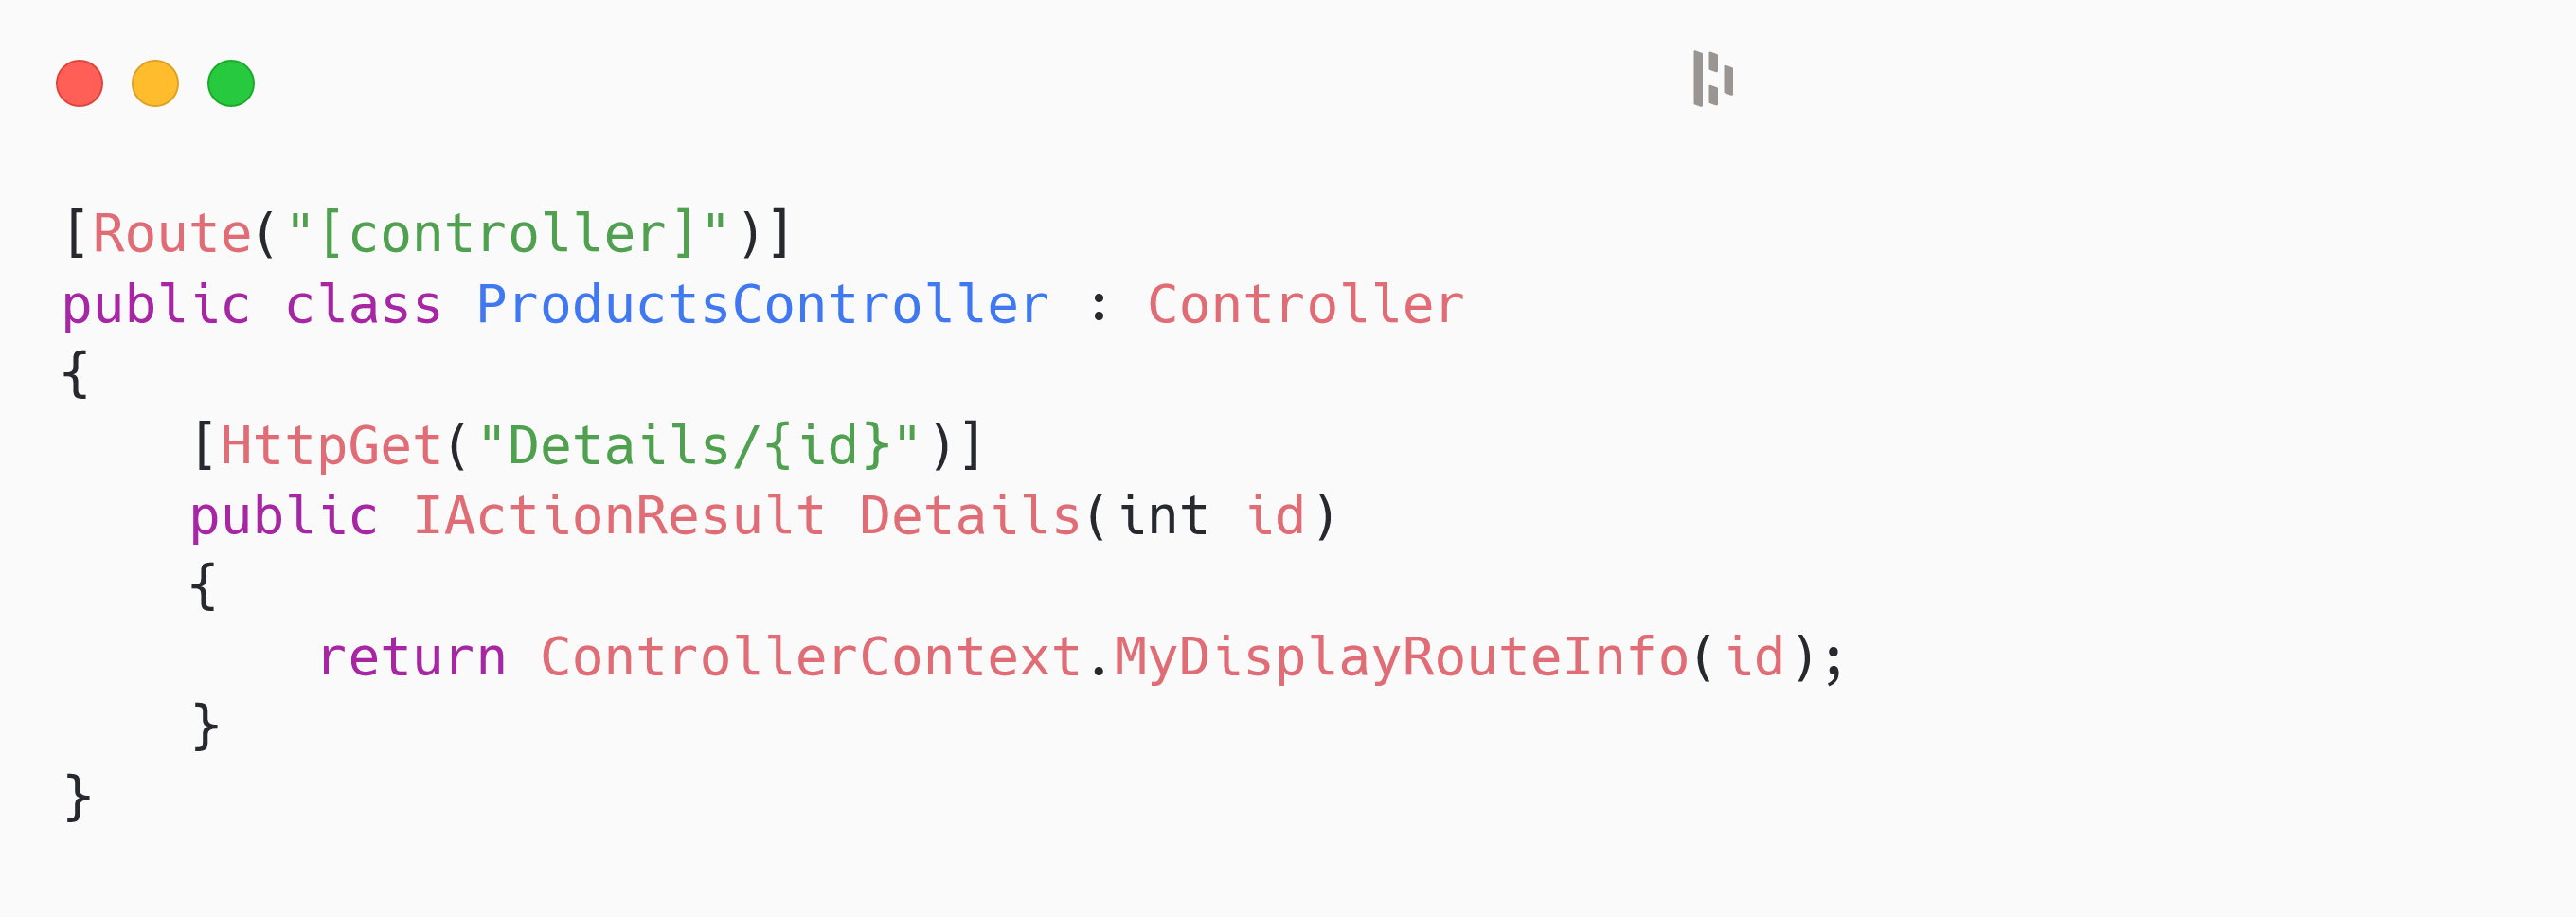
\includegraphics[width=1\textwidth]{graphics/attribute-routing.png}
\caption{An example controller using attributes in ASP.NET Core}
\label{fig:controller}
\end{figure}

In ASP.NET Core, endpoint mapping automation, also known as "action discovery," is achieved by dynamically scanning the entire codebase during the startup phase of the application. However, this dynamic action discovery relies on certain services and middleware incorporated into the application at different stages of the startup phase. Figure \ref{fig:startup-phase} shows the startup phase of an ASP.NET Core application and the order of adding services and middleware.

\begin{figure}[H]
\centering
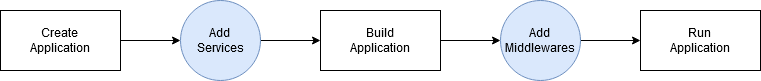
\includegraphics[width=1\textwidth]{graphics/startup-phase.png}
\caption{Flow of the application startup process in ASP.NET Core}
\label{fig:startup-phase}
\end{figure}

ASP.NET Core follows a specific sequence during application setup:

\begin{enumerate}
    \item An application is created, and required services are added to the Dependency Injection (DI) container. Classes can then define their dependencies in their constructor, and the DI container automatically resolves these dependencies to the right implementation.
    \item The application is built, incorporating the registered services.
    \item Middlewares are added. These components have the power to influence how an ASP.NET Core application handles each request.
    \item The application is started.
\end{enumerate}

In this startup sequence, the dynamic action discovery happens before the application is started and involves a middleware and a mapper. The middleware in question is the routing middleware, which relies on the mapper's output to route requests to the correct actions.

The mapper is invoked when using methods like \verb|MapControllers|, which generate the application model—a representation of all controllers and their actions in the application. The process is visualized in Figure \ref{fig:sequence-diagram} as a sequence diagram.

\begin{figure}[H]
\centering
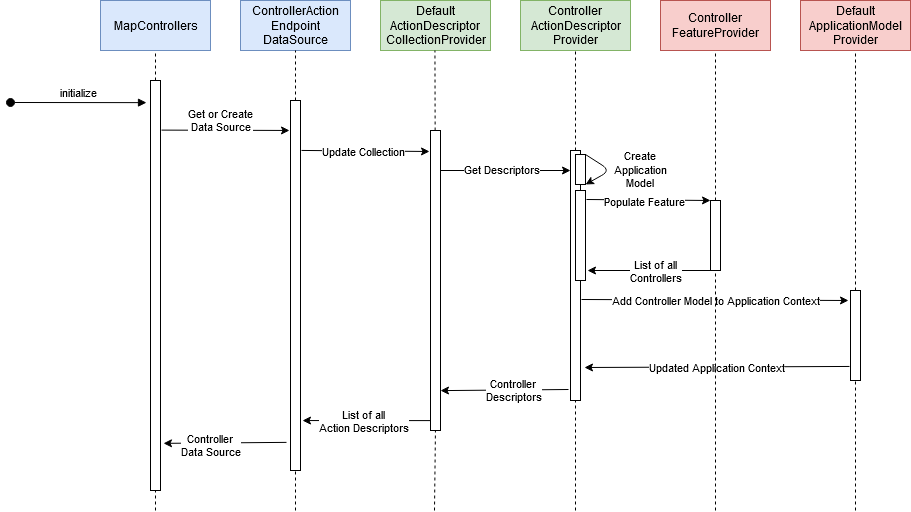
\includegraphics[width=1\textwidth]{graphics/Sequence Diagram.drawio.png}
\caption{Sequence diagram illustrating the application model creation process}
\label{fig:sequence-diagram}
\end{figure}

The sequence of operations leading to action discovery in ASP.NET Core begins when a developer calls the mapping method, such as \verb|MapControllers|. This method, identified in blue in Figure \ref{fig:sequence-diagram}, initiates the process of endpoint mapping.

Upon invocation, \verb|MapControllers| creates an instance of the \verb|ControllerActionEndpointDataSource| (highlighted in blue). This class is responsible for generating a collection of endpoints, which form the building blocks of the application's routing mechanism. Each endpoint encapsulates essential information, such as the target action (method) to be executed upon a specific user request.

In order to generate this collection of endpoints, the \verb|ControllerActionEndpointDataSource| class needs to obtain an overview of all available actions in the application. For this, it requests an \verb|IActionDescriptorCollectionProvider| from the DI container. Per default, this resolves to the \verb|DefaultActionDescriptorCollectionProvider|. It then indirectly calls the \verb|UpdateCollection| method of the \verb|DefaultActionDescriptorCollectionProvider|. This action description provider fetches all the registered \verb|ActionDescriptorProvider| services from the DI container and executes them, thereby gathering actions from a range of sources.

One specific '\verb|ActionDescriptorProvider| service of interest here is the \verb|ControllerActionDescriptorProvider| (marked in green). This service holds the key to our focus area: the actions located within the application's controllers. This service initiates the process of creating an application model—a comprehensive representation of all controller-related information.

The \verb|ControllerActionDescriptorProvider| works through three sequential phases:

\begin{enumerate}
    \item \textbf{Creation of an Application Model}: An empty application model is initialized. This model is designed to hold all relevant information about the controllers in the application and their associated actions.

    \item \textbf{Controller Discovery}: The \verb|ControllerActionDescriptorProvider| calls all available \verb|FeatureProviders| in the DI container, which by default is only the \verb|ControllerFeatureProvider| (marked red). The \verb|ControllerActionDescriptorProvider| then calls the \verb|PopulateFeature| method of every \verb|FeatureProvider| to identify all controllers within the application. The \verb|ControllerFeatureProvider| scans all application parts, which are assemblies that reference the MVC package from ASP.NET Core and could therefore contain controllers. This means that by default, all dependencies that use the MVC package, like Swagger, are analyzed as well. Using reflection, the \verb|PopulateFeature| method analyzes all classes within these assemblies using reflection, extracting those that qualify as controller classes. These discovered controllers are then added to the application model.

    \item \textbf{Model Population}: The \verb|ControllerActionDescriptorProvider| proceeds to call all available \verb|ApplicationModelProviders| in the DI container. These providers populate the application model with detailed information about the actions within each identified controller. The most important \verb|ApplicationModelProvider| is the \verb|DefaultApplicationModelProvider| (marked red) which loops over the found controllers and extracts their actions along with any associated attributes. The service then creates 'selectors' for each action that holds information about the action's route, the HTTP method (GET, POST, DELETE, etc.), a unique name for the action, and other relevant metadata.
\end{enumerate}

After these three phases, the \verb|ControllerActionDescriptorProvider| has effectively created an application model containing all the information about the controllers of the application. This model is sent back up the call stack to the \verb|MapControllers| method, which compiles this information into Endpoint objects. The routing mechanism uses these endpoint objects to appropriately route incoming requests to the correct actions.

The key takeaway is that the services marked in red in Figure \ref{fig:sequence-diagram}—the \verb|ControllerFeatureProvider|, and \verb|DefaultApplicationModelProvider|—play crucial roles in dynamic action discovery and need to be replaced for static action discovery. The objects marked in blue represent objects that are either directly called by the developer or instantiated without dependency injection and can not be modified. The green objects represent services that can be modified by changing the implementation in the DI container but do not use reflection and therefore do not need to be modified by the static action discovery. Optimizing the startup performance of the application involves substituting the services marked red with custom implementations of the same interfaces designed to employ static action discovery. The creation of the static action discovery is the focus of the next chapter.
\chapter{Results}

The results section delves into the performance differences between static and dynamic action discovery methods across three key aspects: startup time, build duration, and memory usage during startup. Each subsequent section provides specific findings, illustrating how varying the number of controllers impacts these metrics and revealing the comparative performance implications of the two action discovery approaches.

\section{Impact on Startup Time}

The assessment of startup time under varying conditions is an integral component of this study. It is important to note that each graph depicts four runs of a benchmark, with each run consisting of 200 iterations. Here, an iteration signifies the duration it takes to start the web server and for it to be ready to process requests.

Figure \ref{fig:dynamic-startup-100} illustrates the startup time for a small application comprising 100 controllers using the existing dynamic action discovery. An observable initial slowdown is noted, with the first run beginning around 21ms and gradually decreasing to around 18.5ms over 200 iterations. However, subsequent runs display a more consistent startup duration ranging between 10 and 11 milliseconds. Overall, the mean startup time of the application employing dynamic action discovery averages 12.55 milliseconds, with an error margin of 0.47 and a standard deviation of 3.95.

\begin{figure}[H]
\centering
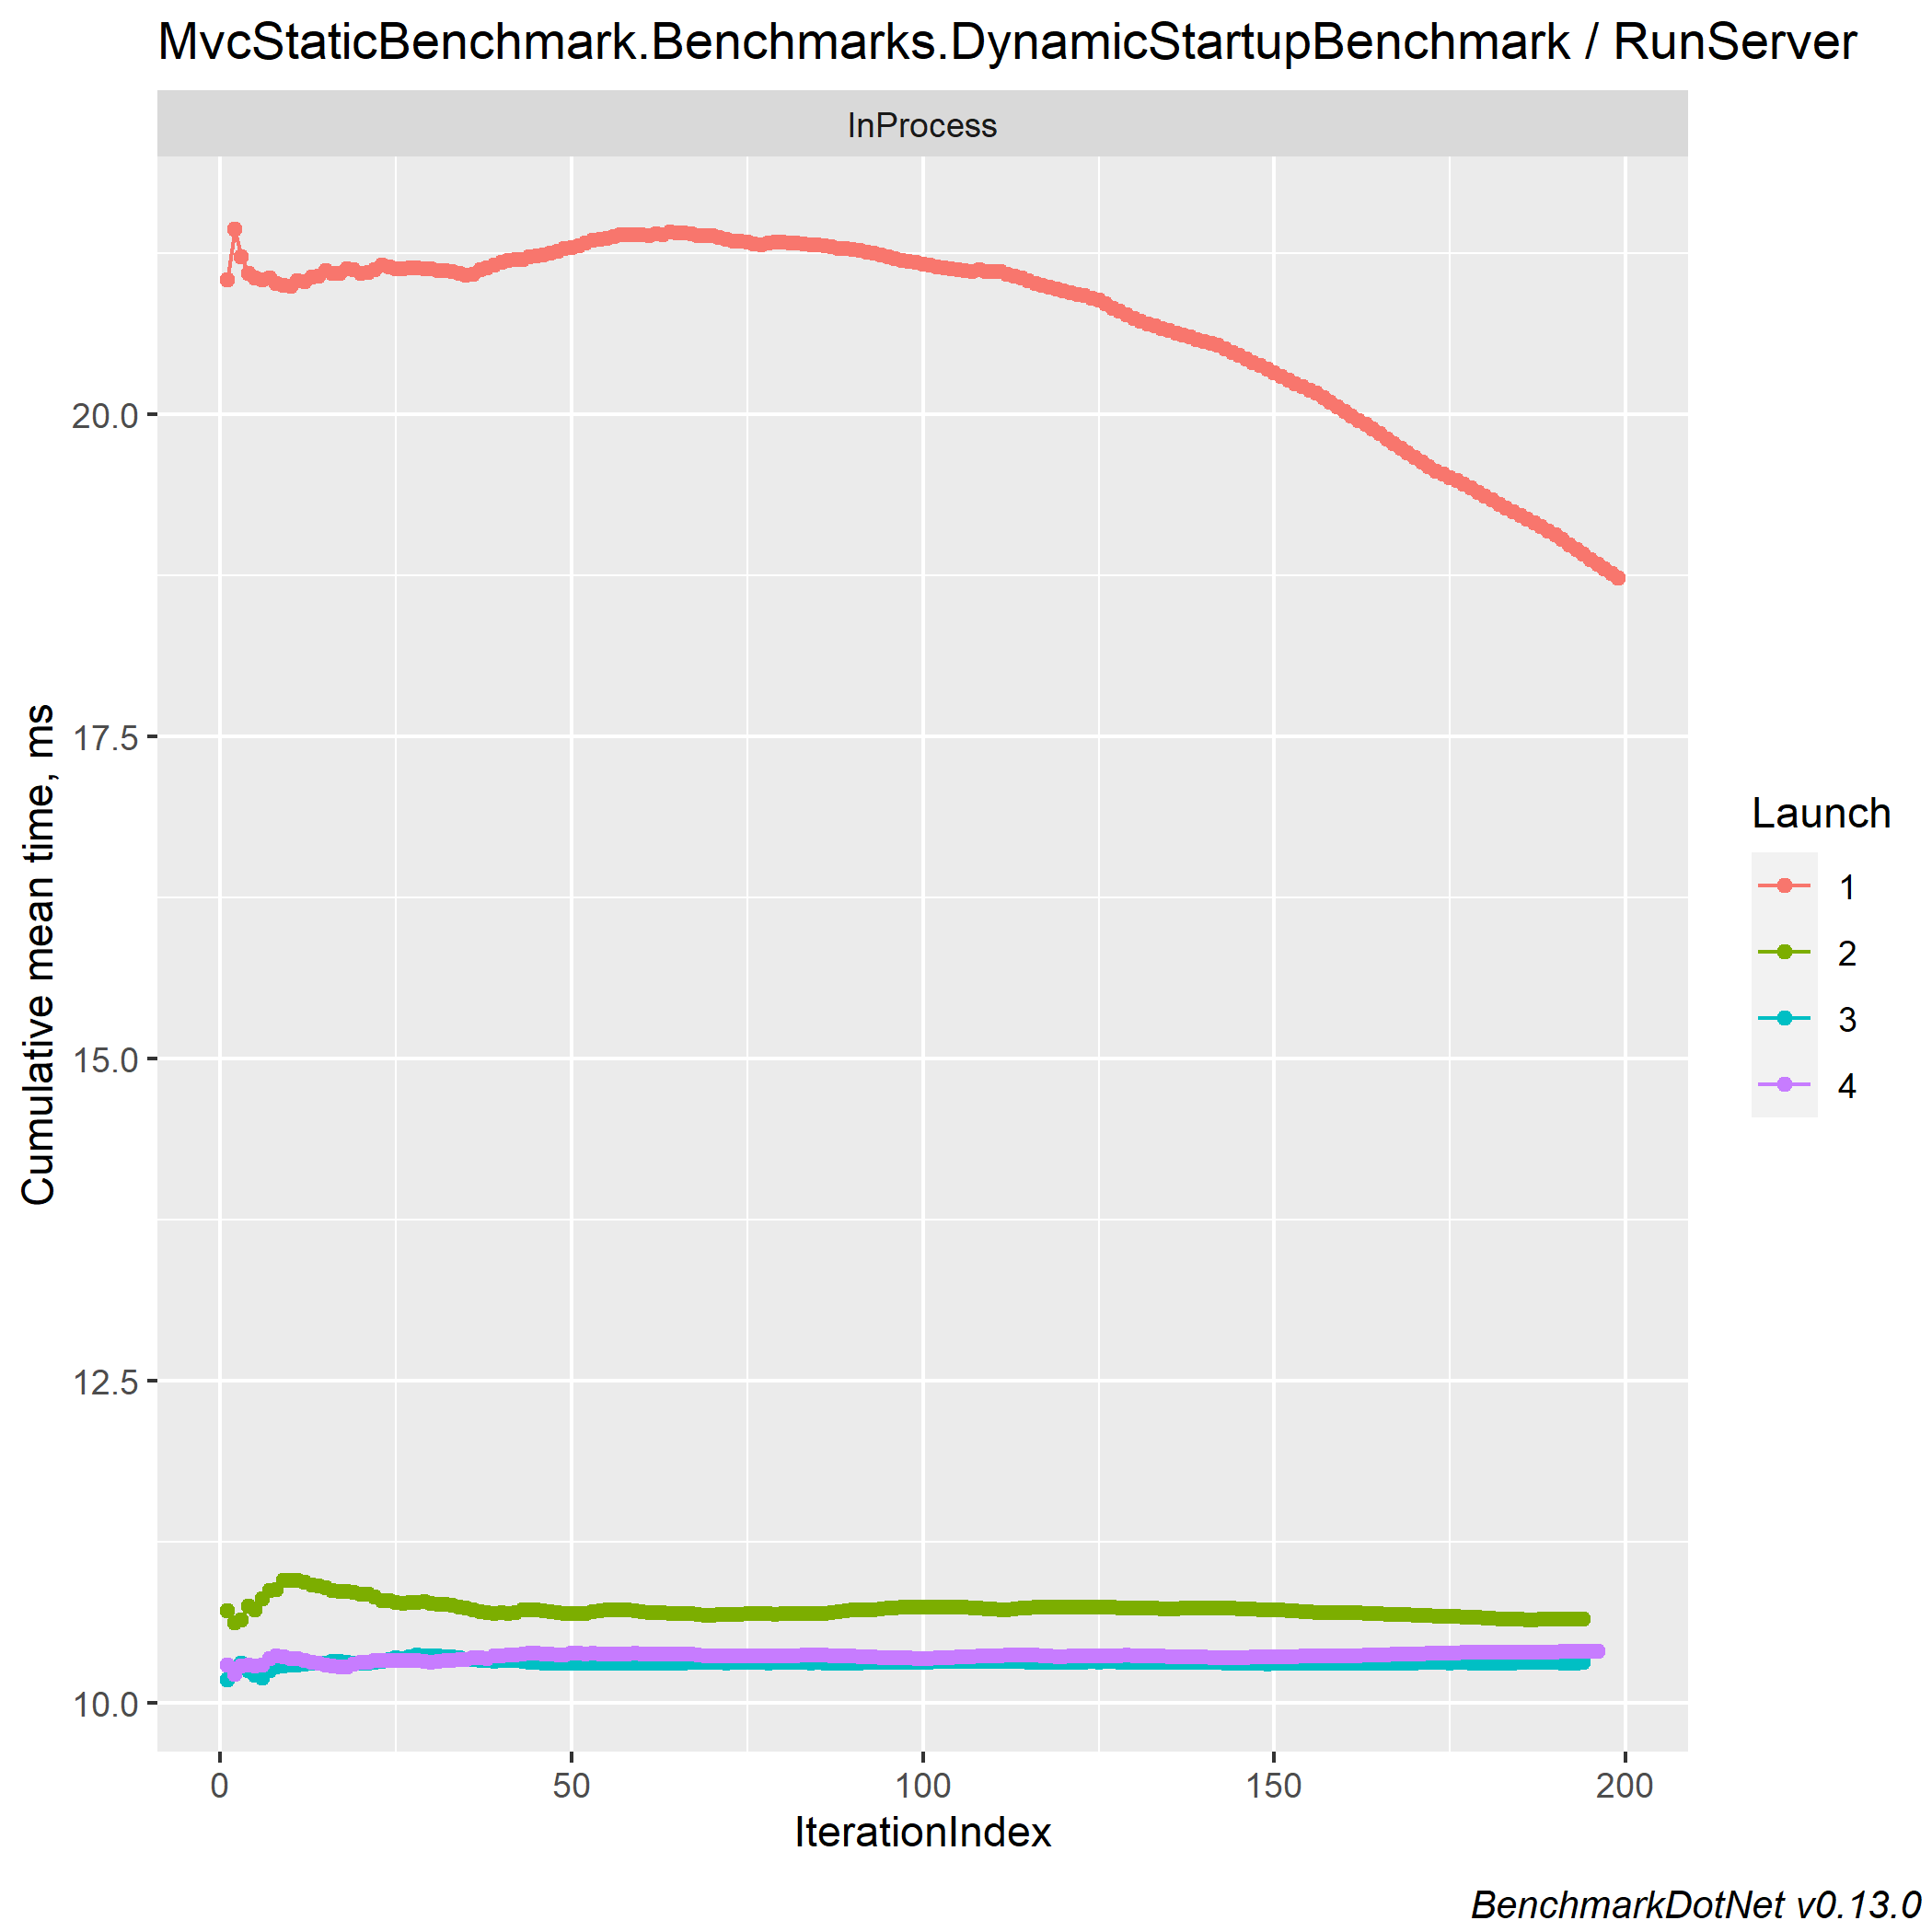
\includegraphics[width=0.8\textwidth]{graphics/MvcStaticBenchmark.Benchmarks.DynamicStartupBenchmark-RunServer-cummean.png}
\caption{Average startup time of an application using dynamic action discovery with 100 controllers}
\label{fig:dynamic-startup-100}
\end{figure}

In contrast, Figure \ref{fig:static-startup-100} presents the same application employing static action discovery. Here, the first two runs average around 6.5 milliseconds, while the last two runs maintain a consistent speed of approximately 3 milliseconds. This setup results in a mean startup time of 4.68 milliseconds, an error margin of 0.19, and a standard deviation of 1.59.

\begin{figure}[H]
\centering
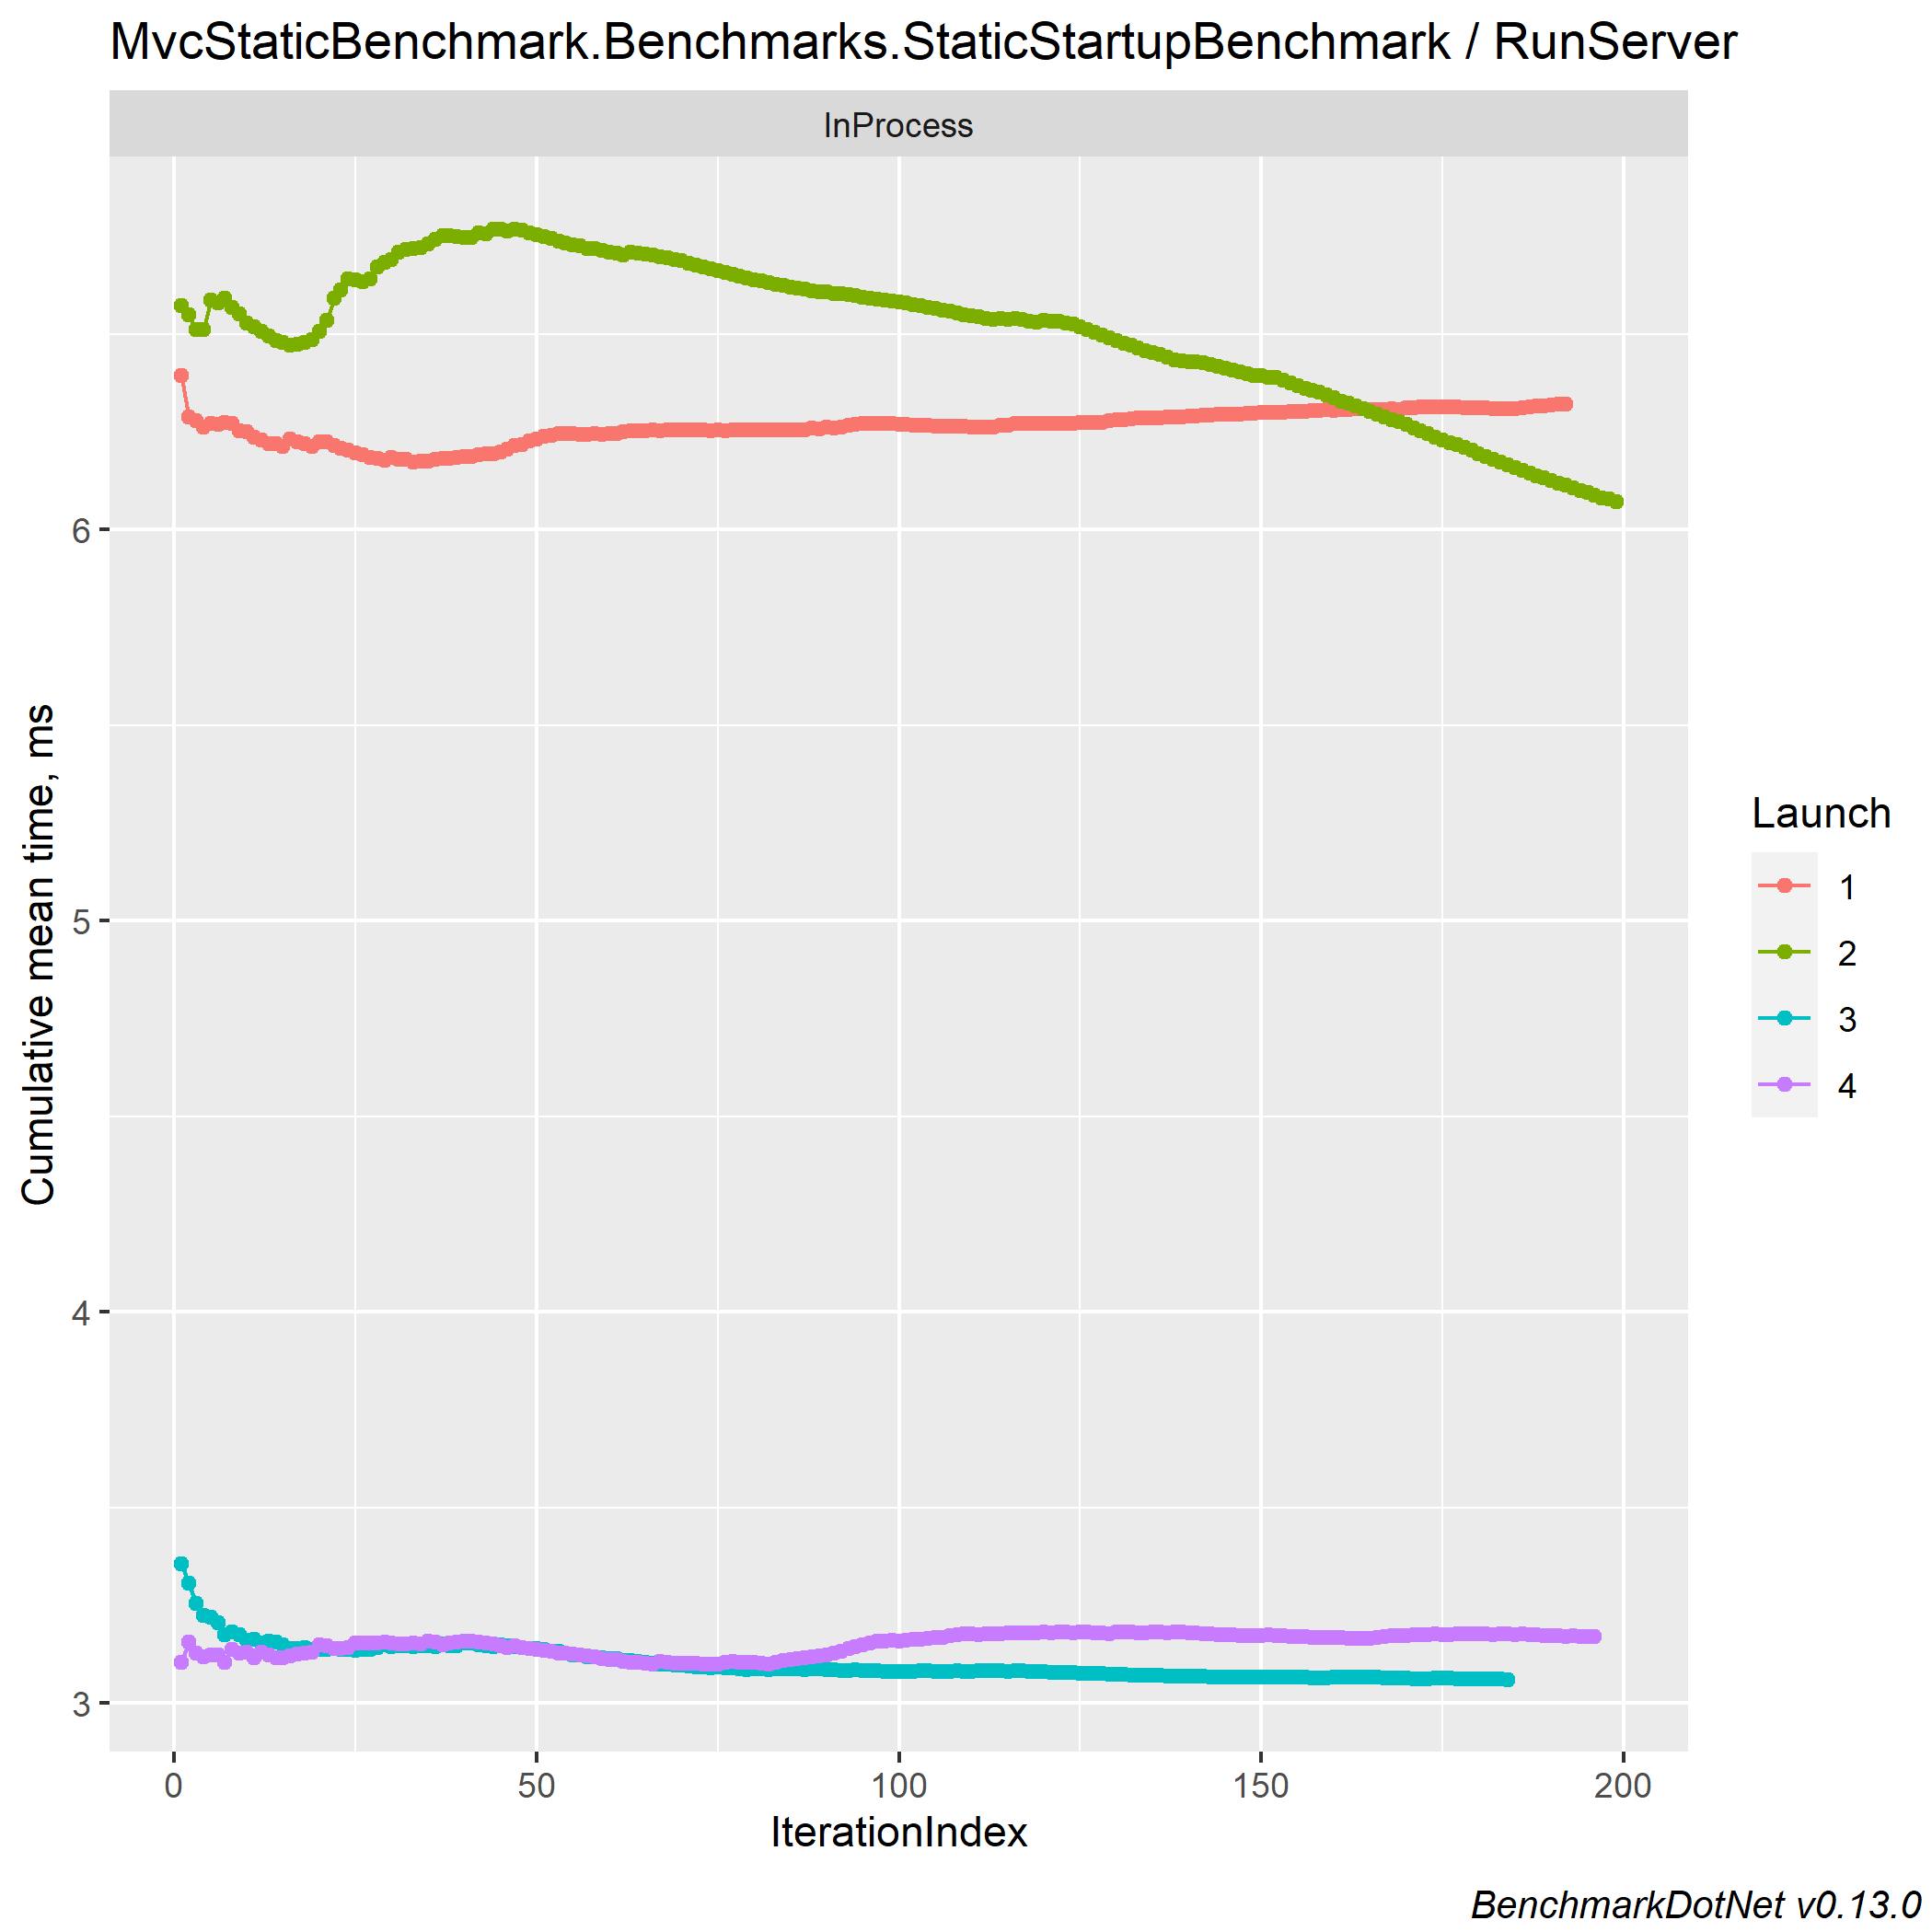
\includegraphics[width=0.8\textwidth]{graphics/MvcStaticBenchmark.Benchmarks.StaticStartupBenchmark-RunServer-cummean.png}
\caption{Average startup time of an application using static action discovery with 100 controllers}
\label{fig:static-startup-100}
\end{figure}

Expanding the application size to include 1,000 controllers, the startup time under dynamic action discovery (Figure \ref{fig:dynamic-startup-1000}) appears relatively turbulent at the beginning of each benchmark. However, the measurements eventually stabilize around 86 milliseconds. The mean startup time for this application under dynamic action discovery is 86.02 milliseconds, with an error margin of 0.14 and a standard deviation of 1.16.

\begin{figure}[H]
\centering
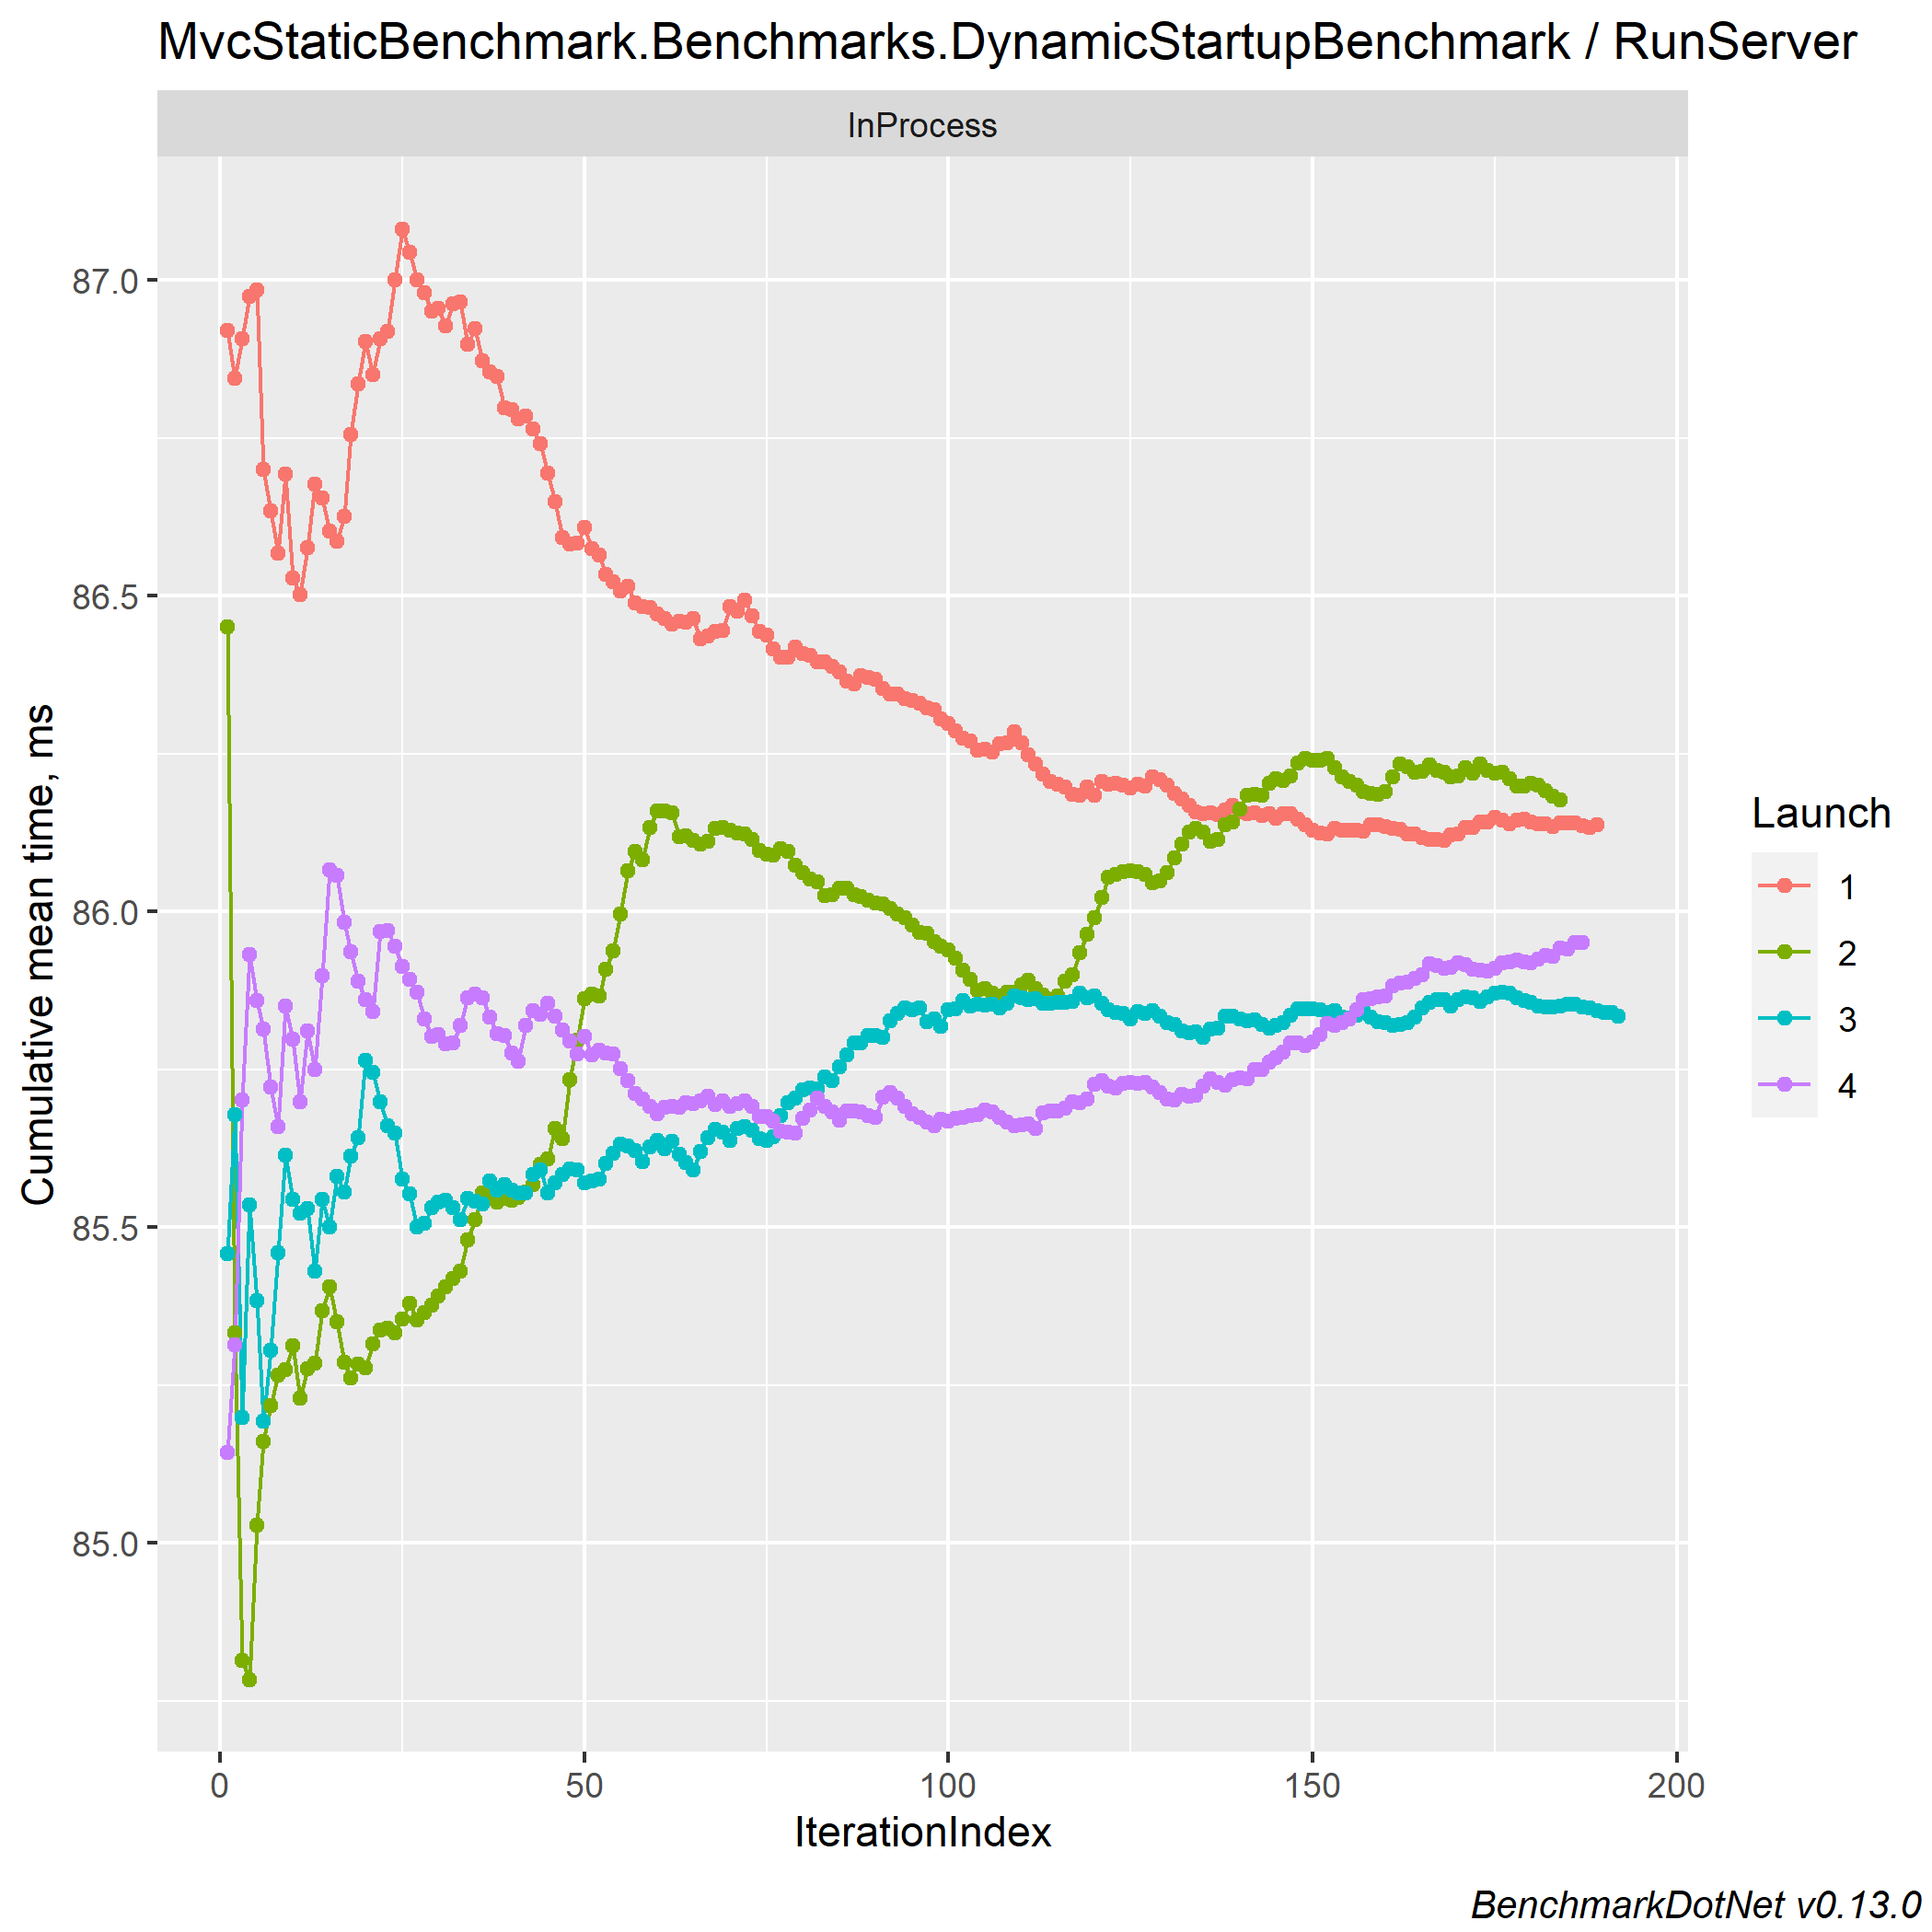
\includegraphics[width=0.8\textwidth]{graphics/MvcStaticBenchmark.Benchmarks.DynamicStartupBenchmark-RunServer-cummean 1000.png}
\caption{Average startup time of an application using dynamic action discovery with 1000 controllers}
\label{fig:dynamic-startup-1000}
\end{figure}

Figure \ref{fig:static-startup-1000} portrays the static action discovery approach for the same 1,000 controller application. Here, we observe two distinct groups of runs: the first two runs average between 16.2 and 17 milliseconds, while the latter two consistently fall between 15 and 15.7 milliseconds. The mean duration is 15.9 milliseconds, with an error of 0.084 and a standard deviation of 0.706.

\begin{figure}[H]
\centering
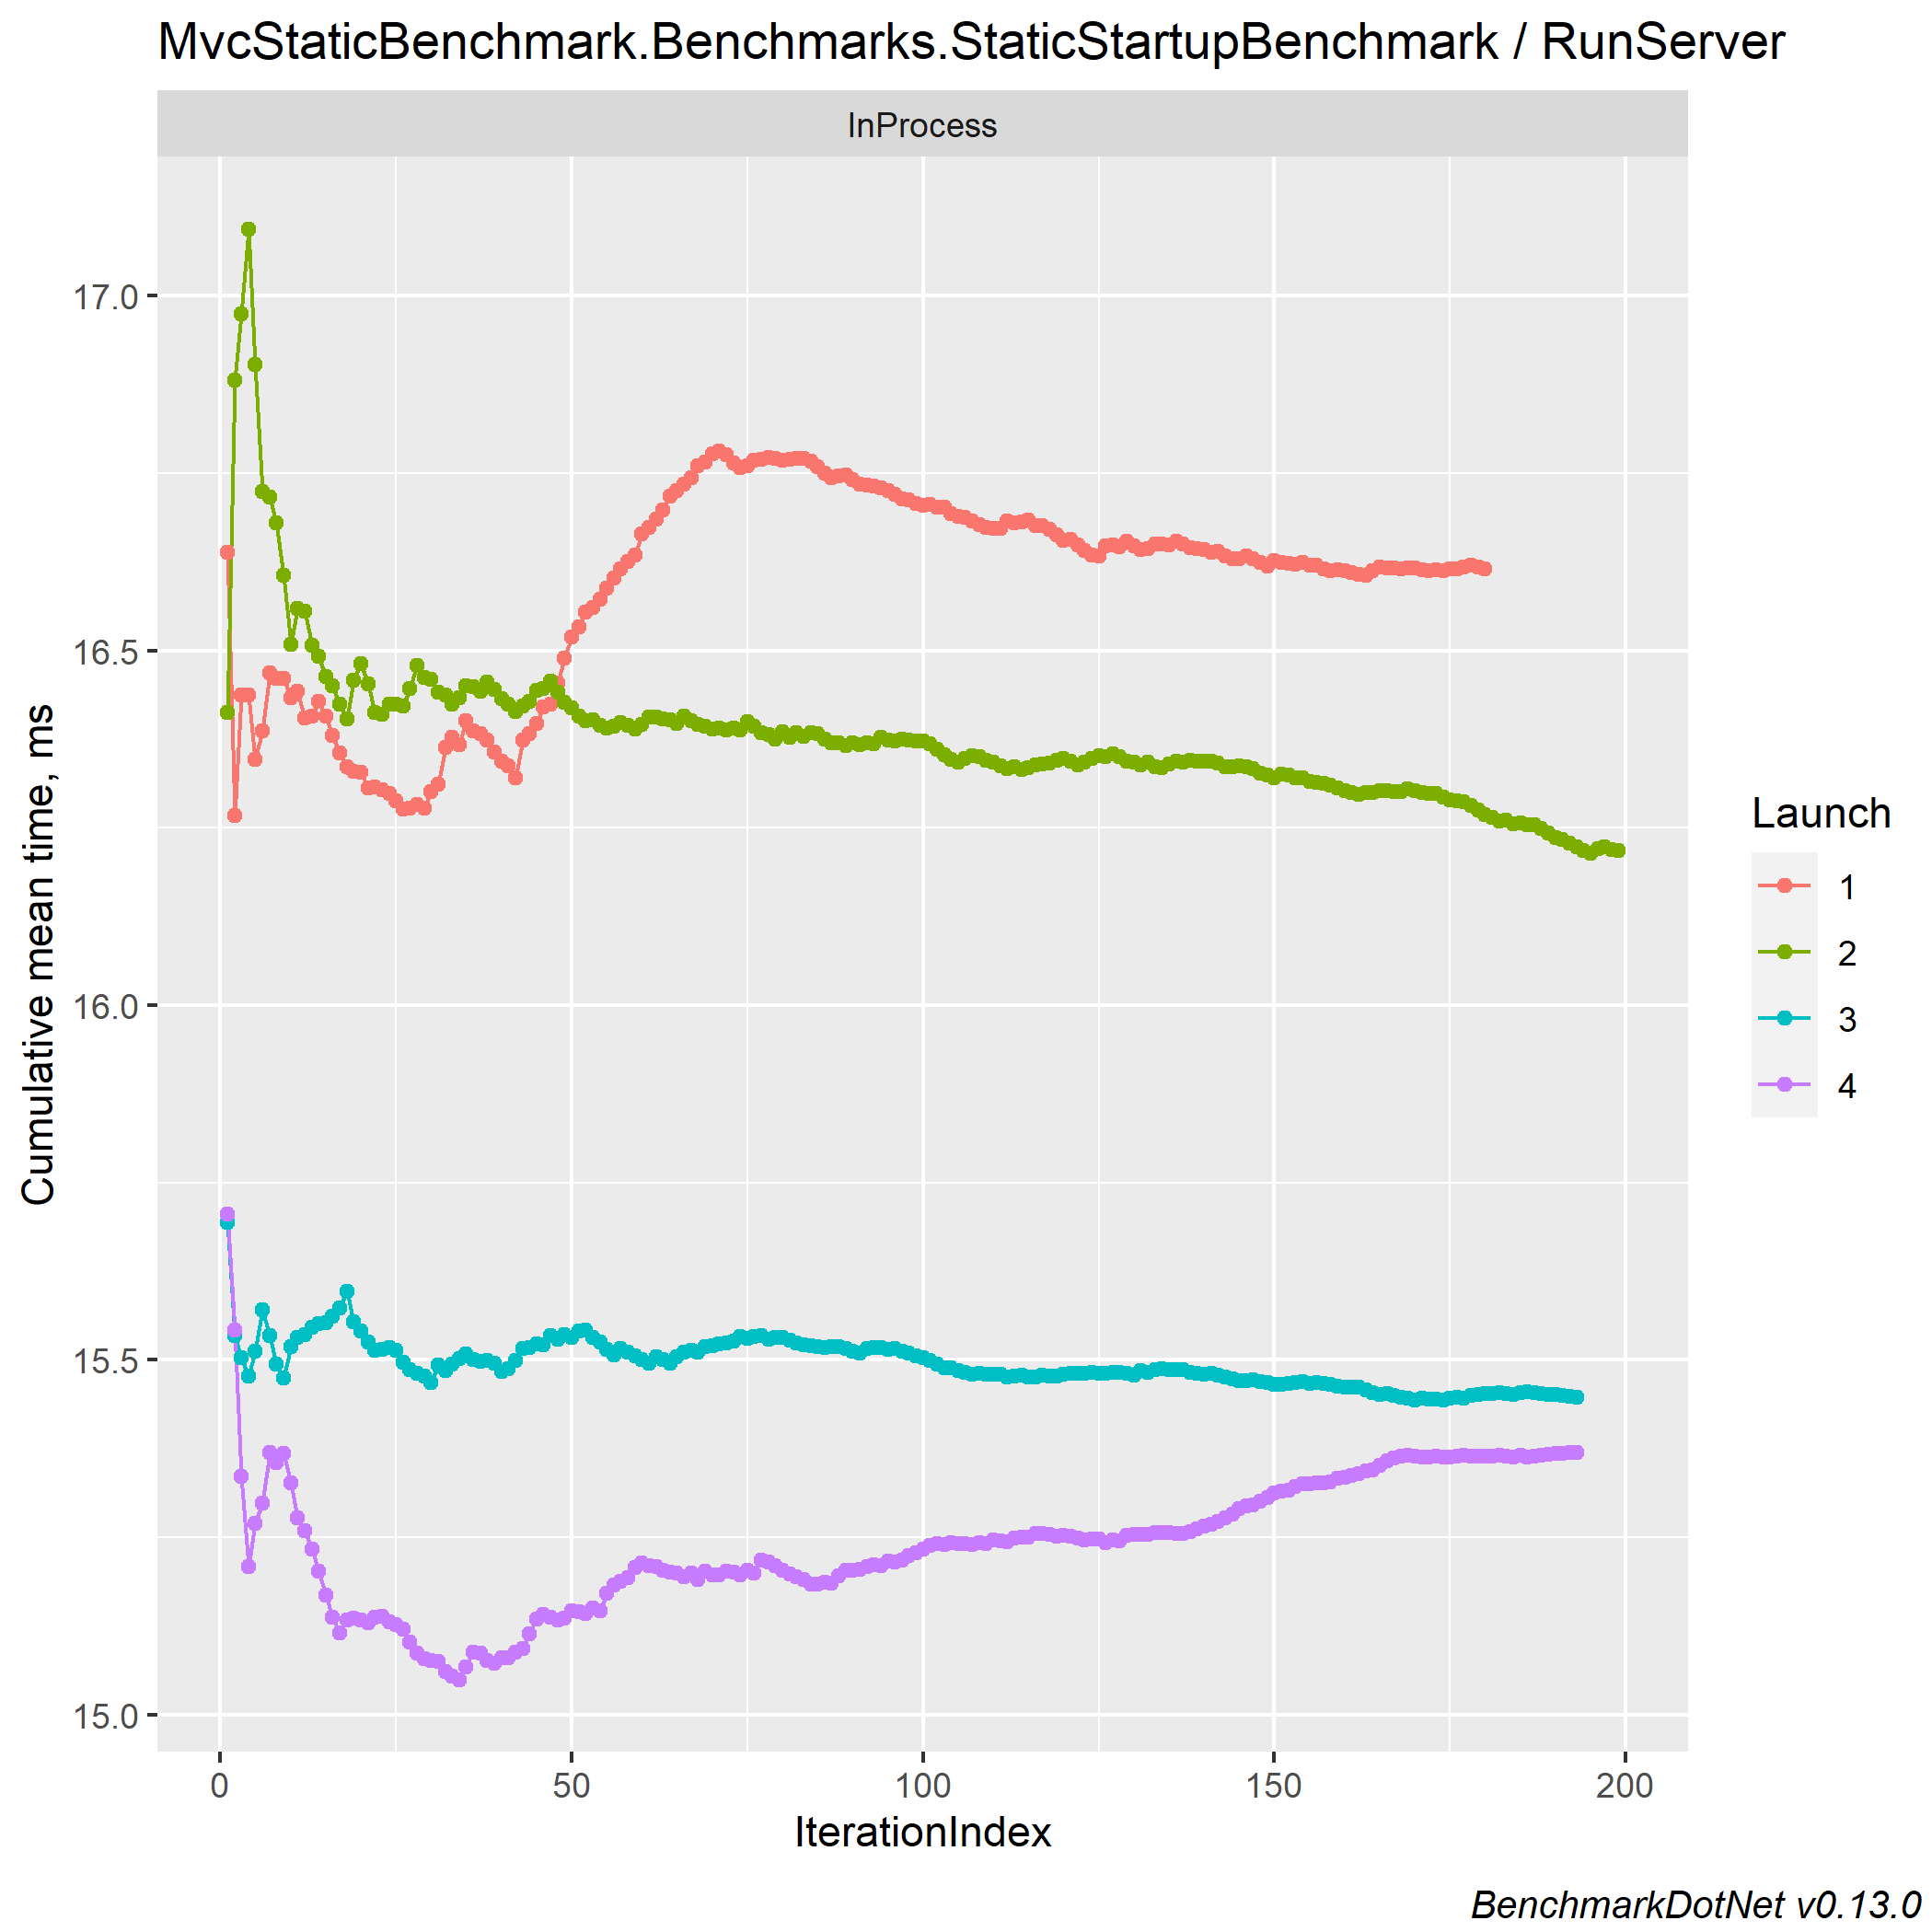
\includegraphics[width=0.8\textwidth]{graphics/MvcStaticBenchmark.Benchmarks.StaticStartupBenchmark-RunServer-cummean 1000.png}
\caption{Average startup time of an application using static action discovery with 1000 controllers}
\label{fig:static-startup-1000}
\end{figure}

Increasing the controller count to 10,000, dynamic action discovery (Figure \ref{fig:dynamic-startup-10000}) results in a fluctuation between 880 and 900 milliseconds at the outset, which ultimately stabilizes around 887 milliseconds. However, the fourth run deviates, rising to 910 milliseconds before settling to 900 milliseconds. Averaging across the four runs, the mean time is 890.6 milliseconds, with an error of 1.48 and a standard deviation of 12.41.

\begin{figure}[H]
\centering
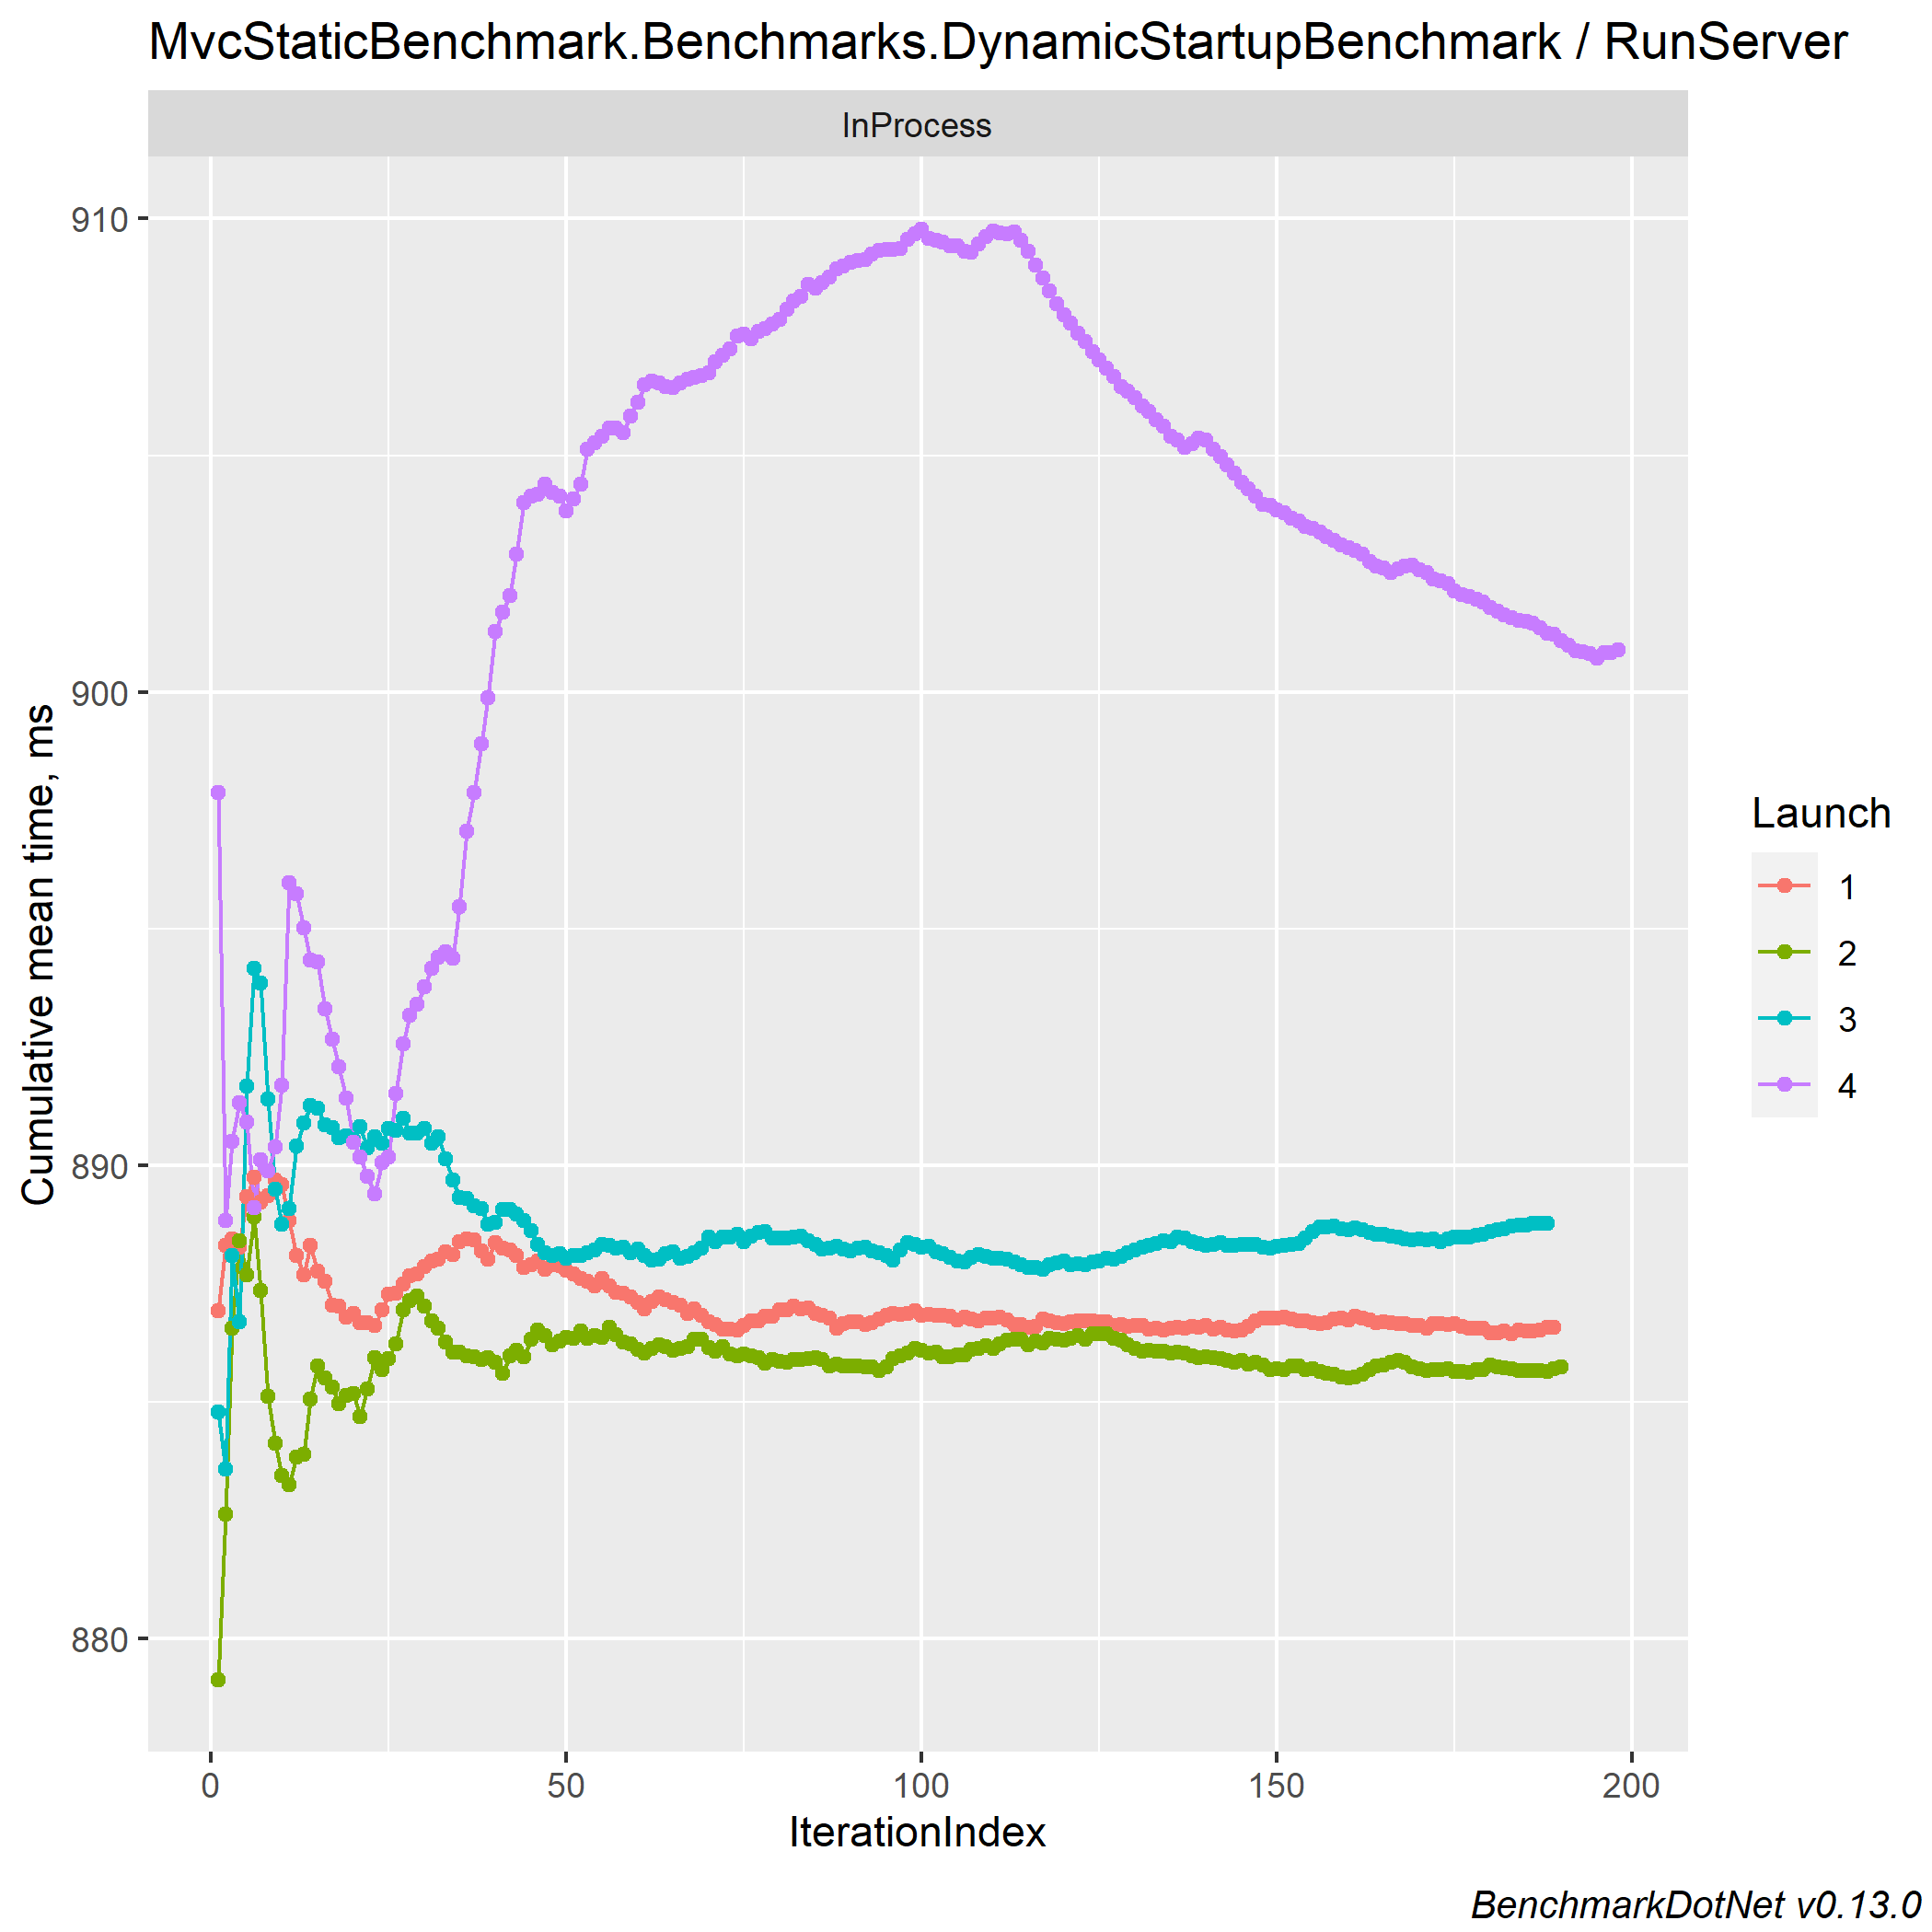
\includegraphics[width=0.8\textwidth]{graphics/MvcStaticBenchmark.Benchmarks.DynamicStartupBenchmark-RunServer-cummean 10 000.png}
\caption{Average startup time of an application using dynamic action discovery with 10,000 controllers}
\label{fig:dynamic-startup-10000}
\end{figure}

Finally, Figure \ref{fig:static-startup-10000} exhibits the startup times with static action discovery for the 10,000 controller application. The four runs initiate between 193 and 213 milliseconds, converging closer to between 197 and 207 milliseconds by the end. This benchmark presents a mean startup duration of 202 milliseconds, an error of 0.67, and a standard deviation of 5.68.

\begin{figure}[H]
\centering
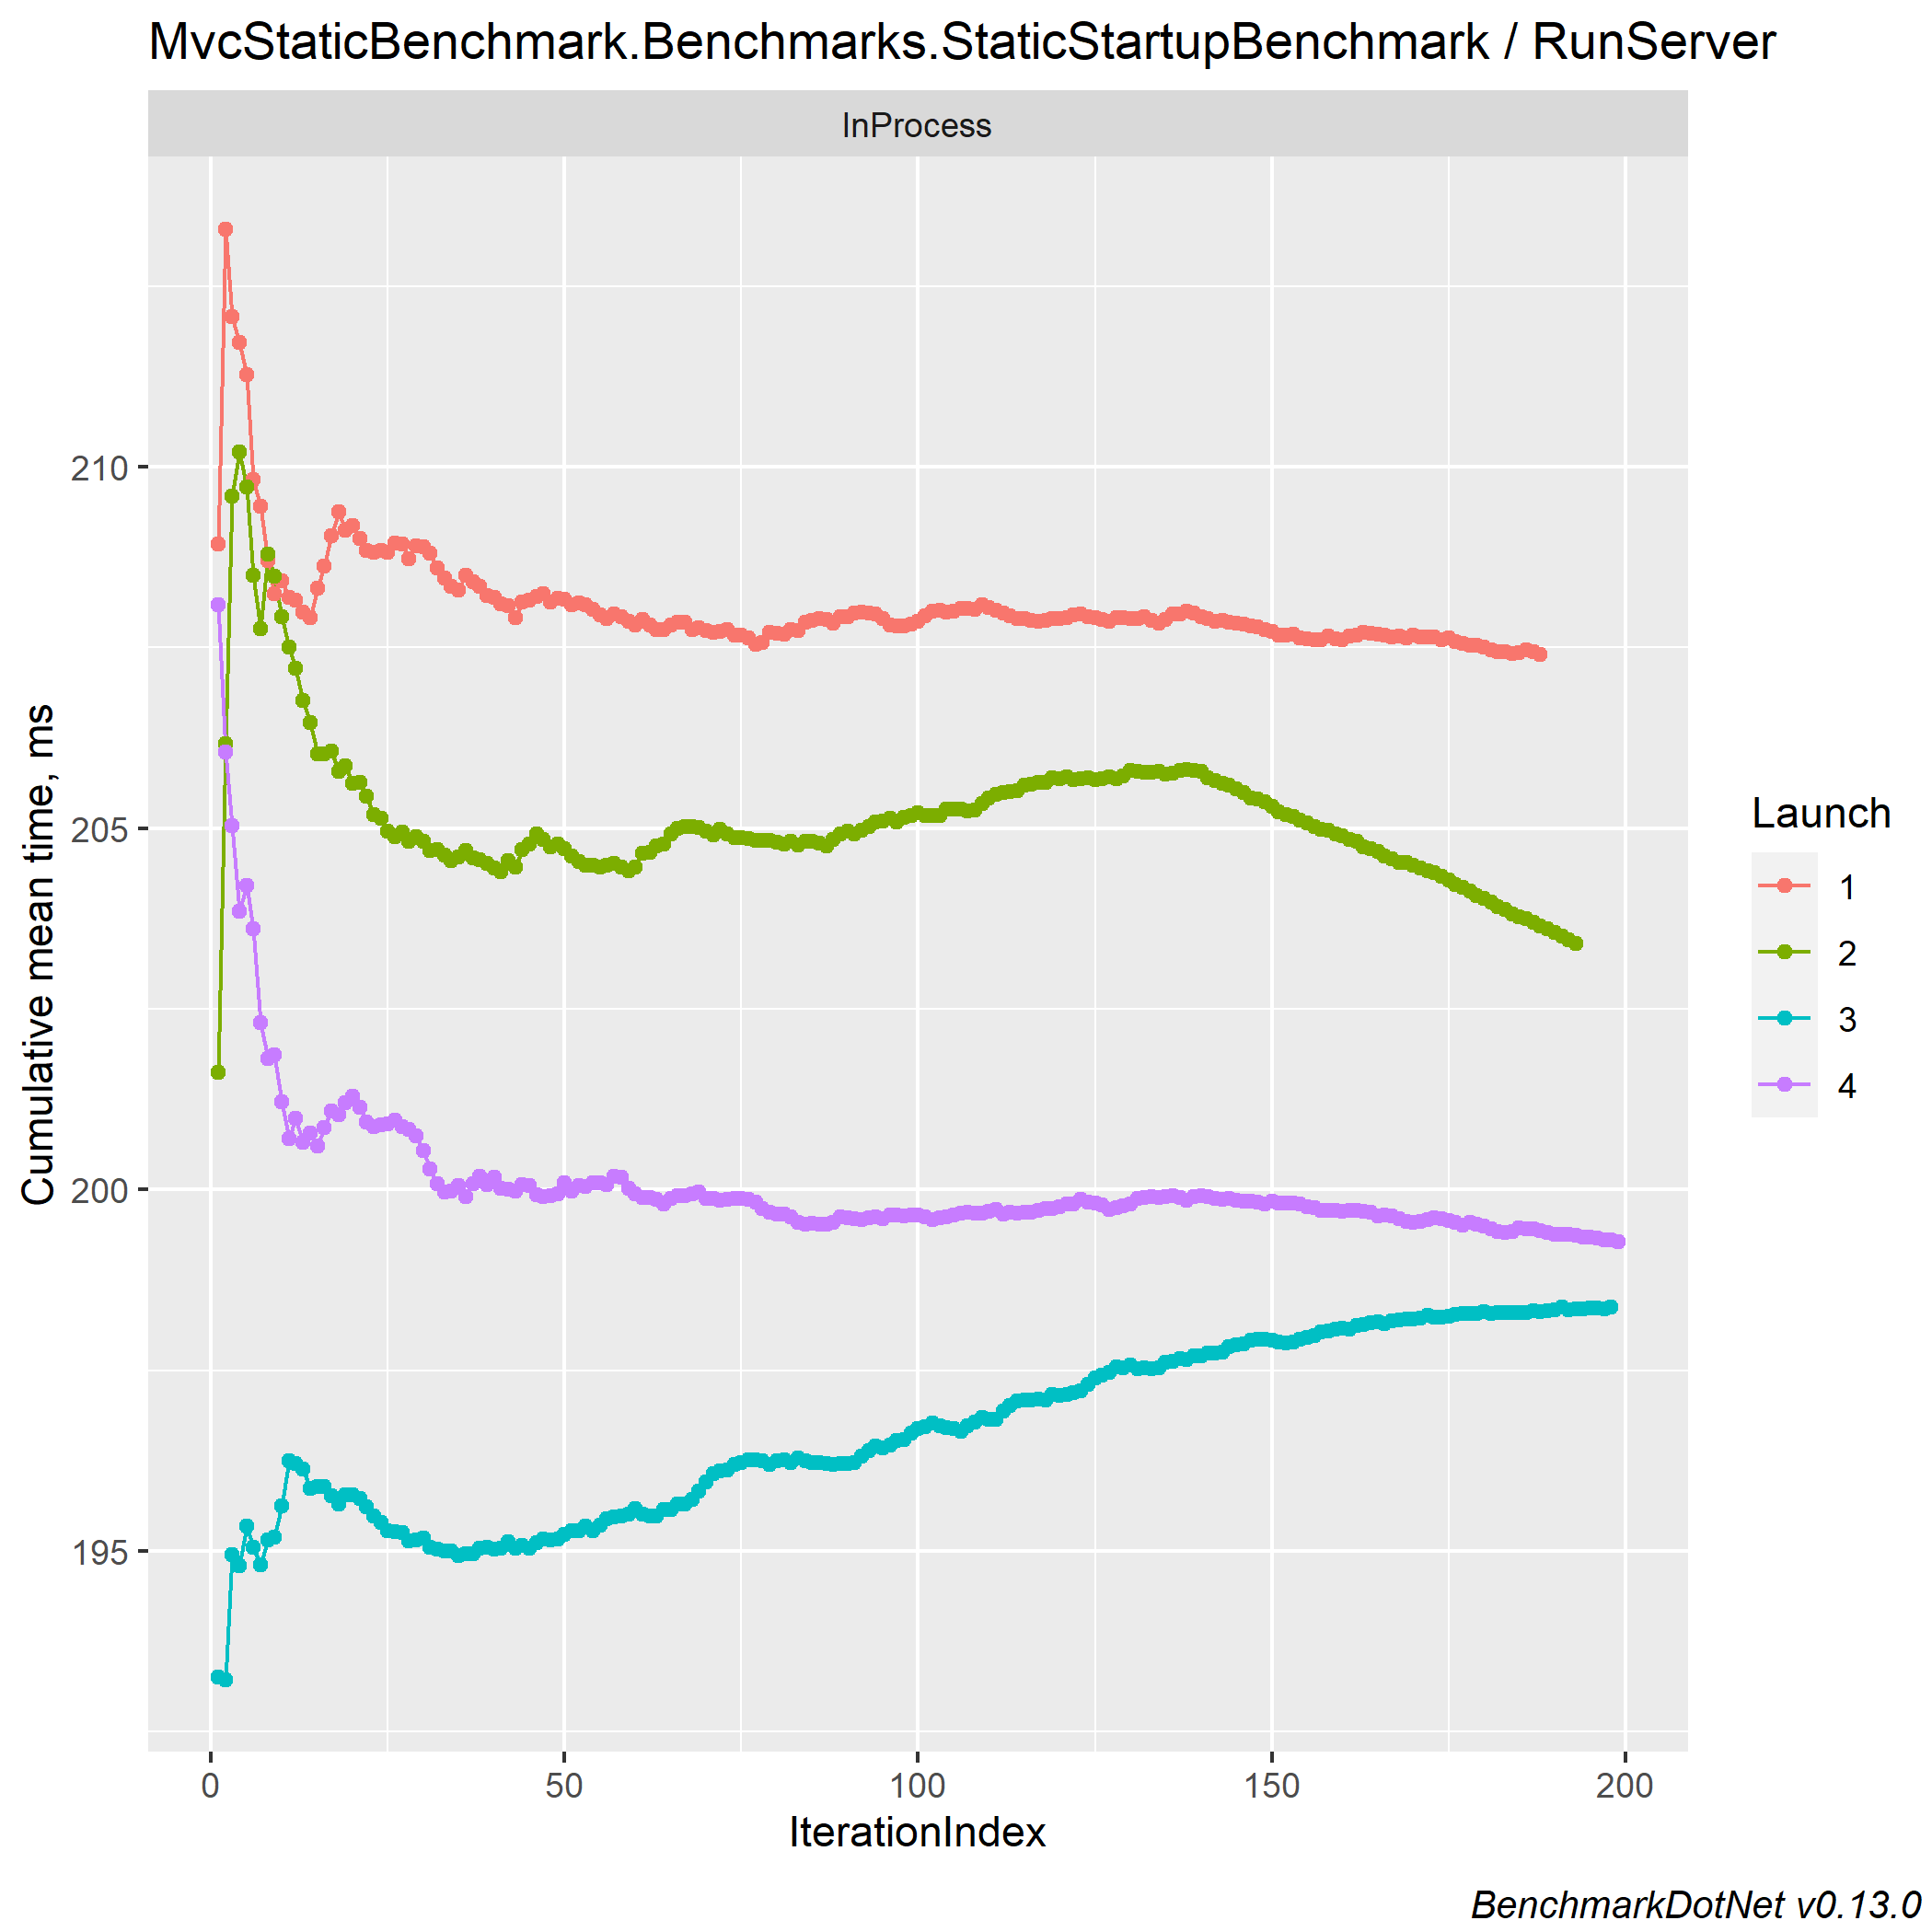
\includegraphics[width=0.8\textwidth]{graphics/MvcStaticBenchmark.Benchmarks.StaticStartupBenchmark-RunServer-cummean 10 000.png}
\caption{Average startup time of an application using static action discovery with 10,000 controllers}
\label{fig:static-startup-10000}
\end{figure}

Furthermore, Figure \ref{fig:startup-time-results} visualizes the mean startup time as a bar chart, with groups representing applications of 100, 1,000, or 10,000 controllers. Each group comprises the mean startup times of both static (right) and dynamic (left) action discoveries. This visualization simplifies comparisons between the methods across varying application sizes.

\begin{figure}[H]
\centering
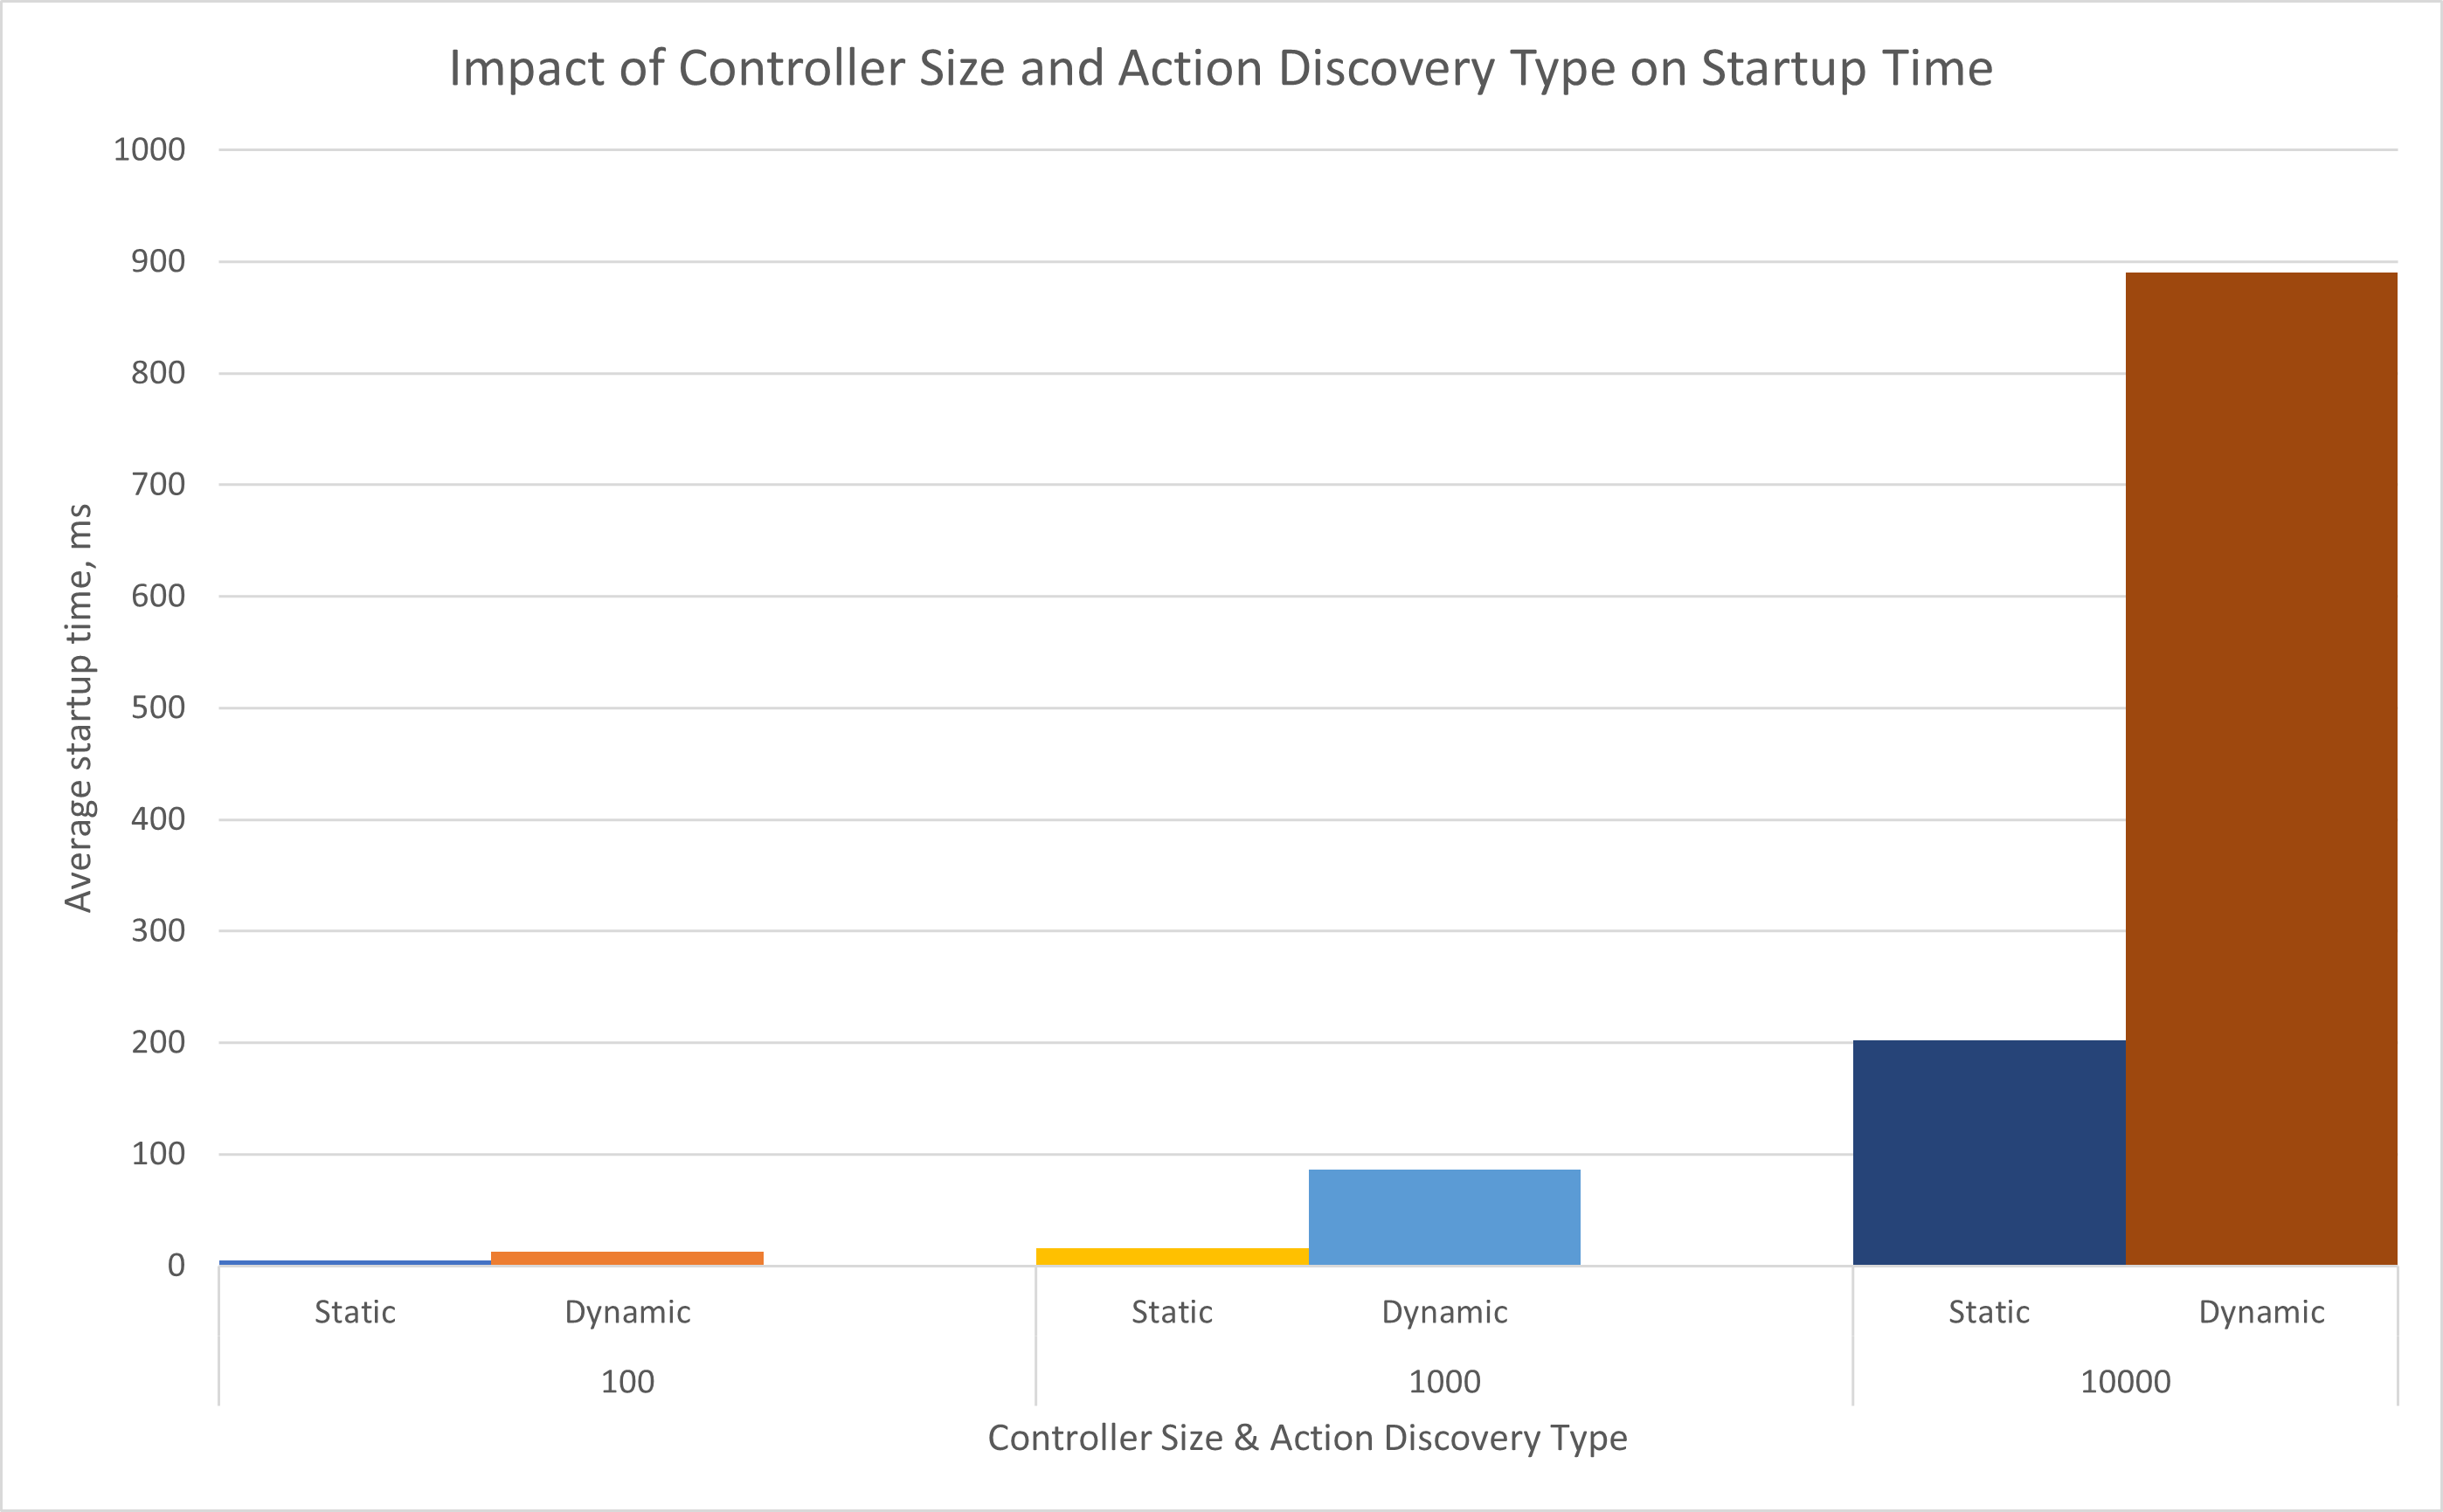
\includegraphics[width=0.8\textwidth]{graphics/Impact of Controller Size and Action Discovery Type on Startup Time.png}
\caption{Impact of Controller Size and Action Discovery Type on Startup Time}
\label{fig:startup-time-results}
\end{figure}

\section{Impact on Build Duration}

The duration of the build process is another significant metric in this analysis. The data reveals that the build time increases exponentially with the number of controllers present in the application.

For an application with 100 controllers utilizing static action discovery, the mean build time was recorded as 1888 milliseconds. Across the 100 measurements, this mean time demonstrated an error of 135 and a standard deviation of 398. By comparison, the same application using dynamic action discovery averaged a shorter build time of 1566 milliseconds, with an error of 24 and a standard deviation of 71.

Escalating to an application size of 1,000 controllers, the mean build time for the static action discovery variant was 4162 milliseconds. This result was associated with an error of 102 and a standard deviation of 302. On the other hand, the dynamic action discovery method posted an average build time of 1779 milliseconds, with an error of 28 and a standard deviation of 81.

Finally, the largest application with 10,000 controllers was analyzed. Here, the static action discovery approach resulted in an average build time of 47276 milliseconds, accompanied by an error of 881 and a standard deviation of 2599. In contrast, employing dynamic action discovery resulted in a significantly lower mean build time of 5843 milliseconds, along with an error of 66 and a standard deviation of 196.

Figure \ref{fig:build-time-results} visually represents these results as a bar chart, categorized by the number of controllers in each application. Within each group, the static action discovery value is displayed on the right, while the dynamic action discovery value is presented on the left. This arrangement allows for an intuitive comparison of build times between the two methods across applications of varying sizes.

\begin{figure}[H]
\centering
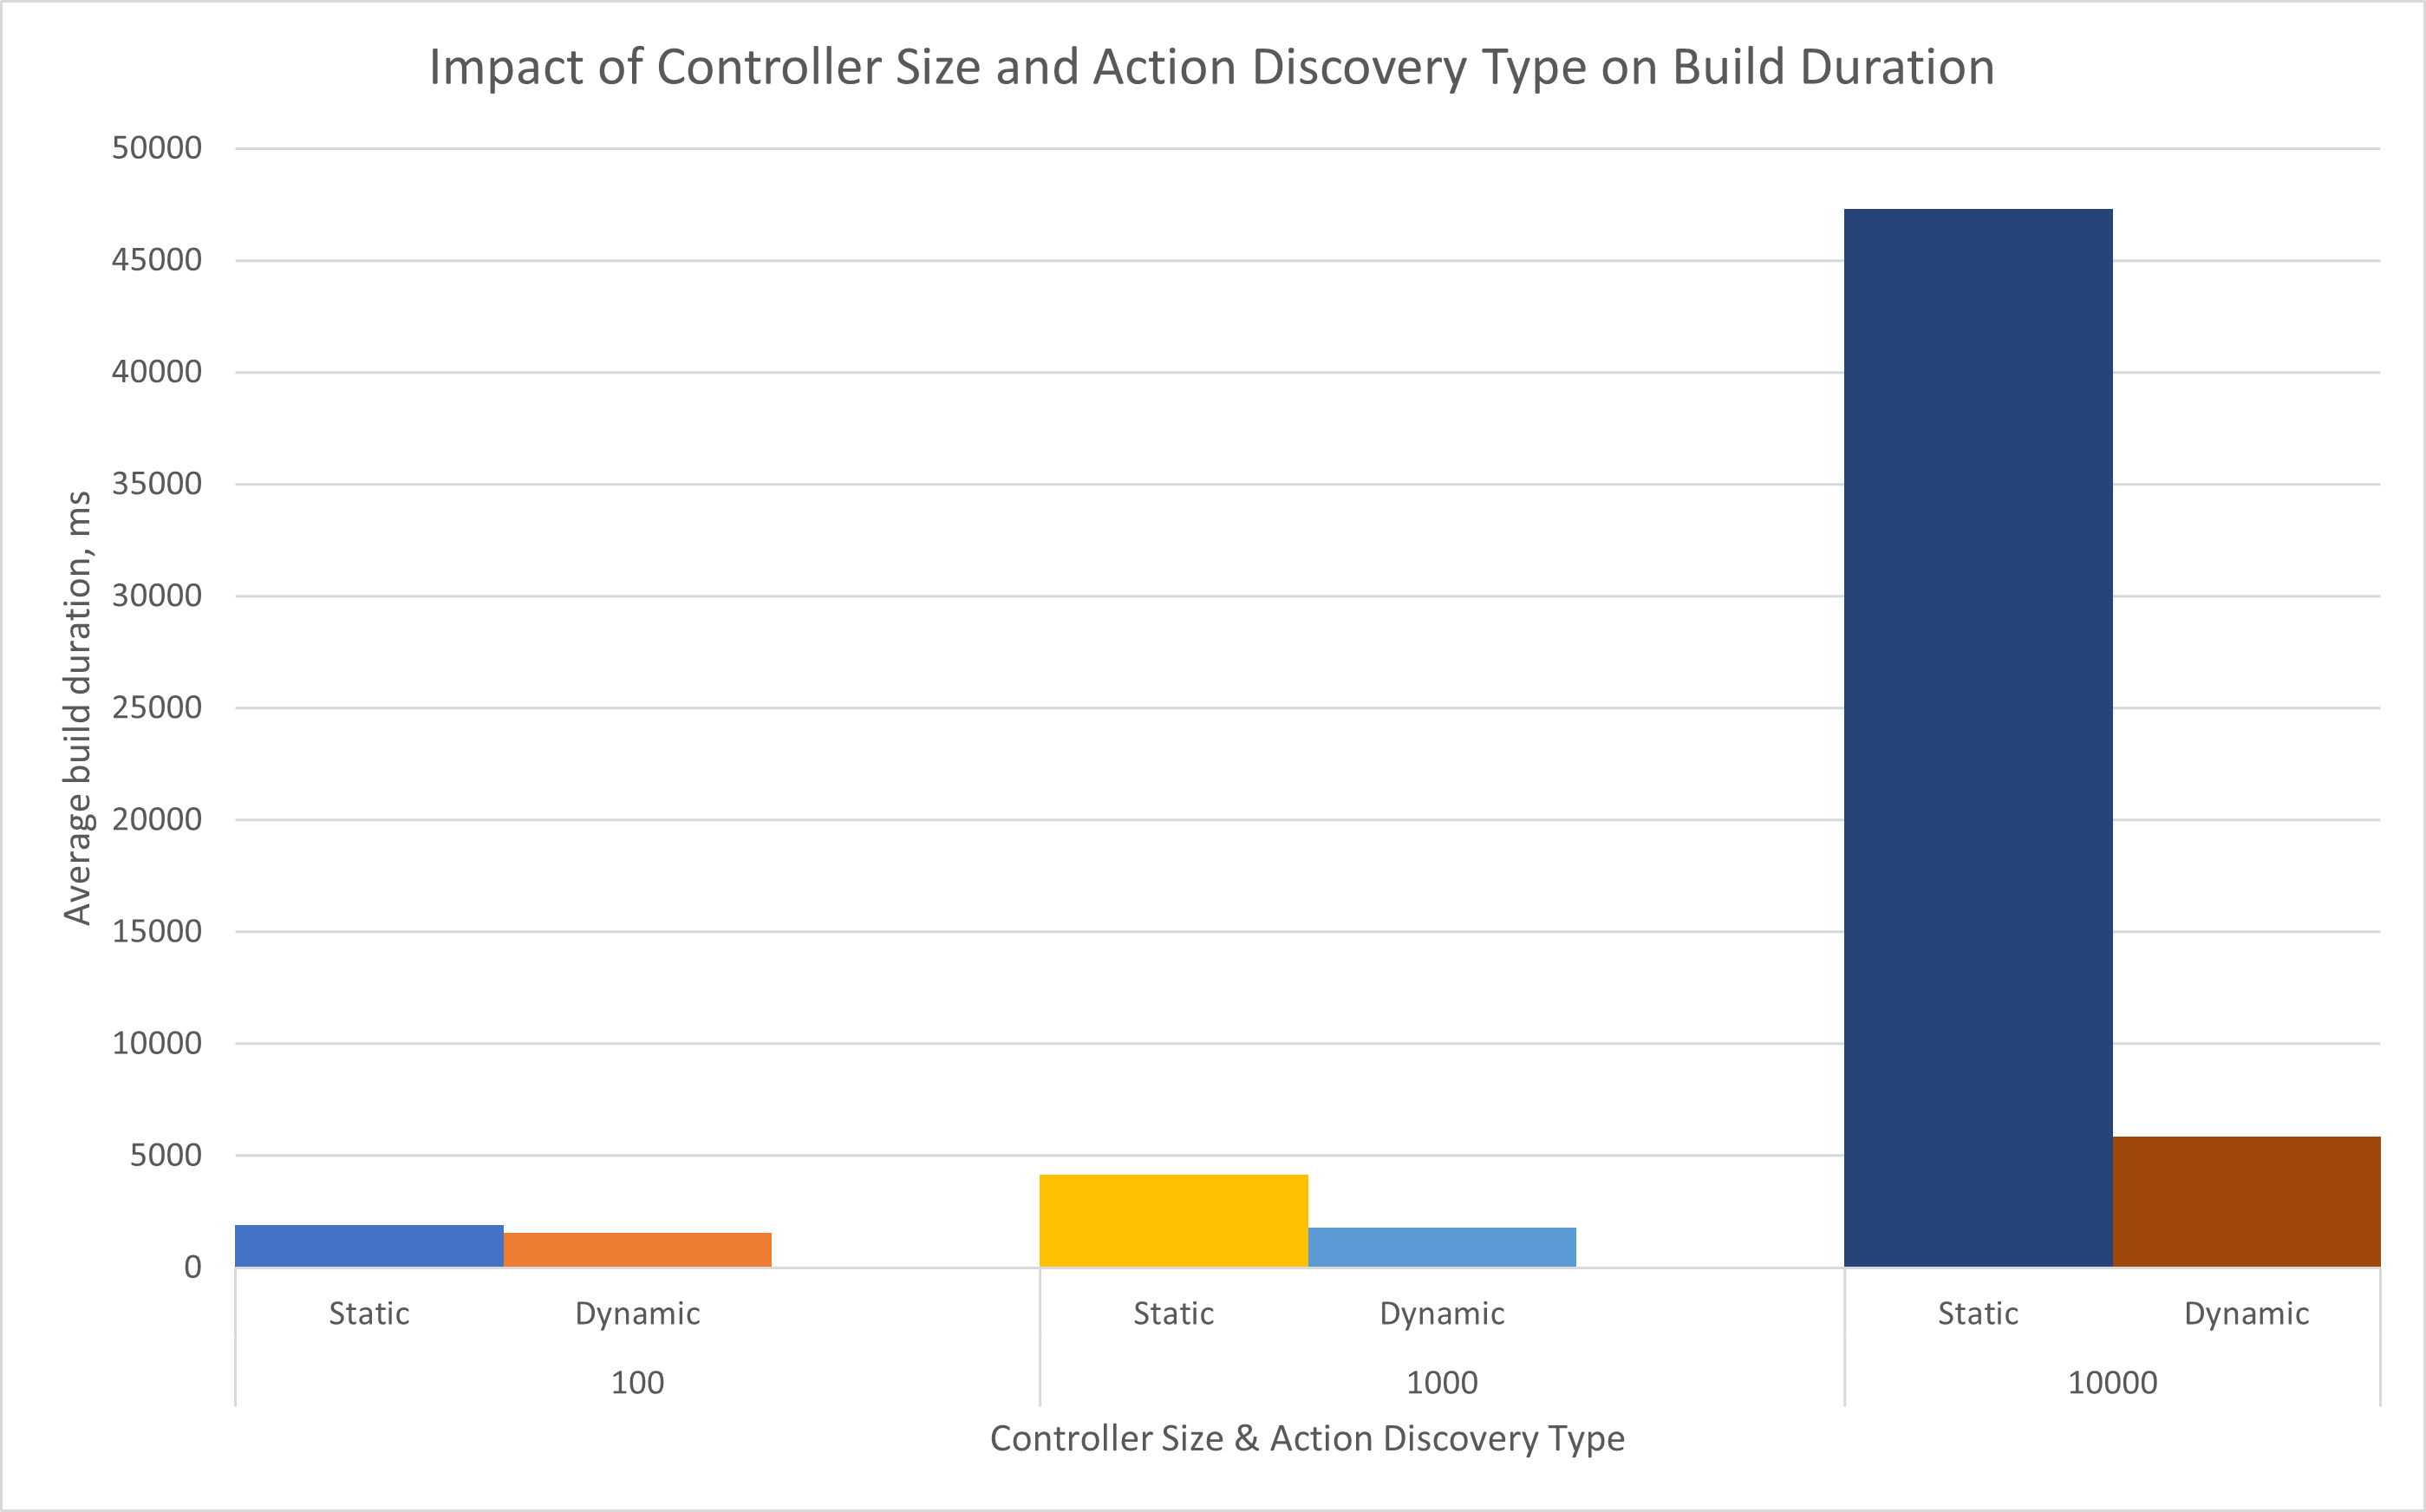
\includegraphics[width=0.8\textwidth]{graphics/Impact of Controller Size and Action Discovery Type on Build Duration.png}
\caption{Impact of Controller Size and Action Discovery Type on Build Duration}
\label{fig:build-time-results}
\end{figure}

\section{Impact on Memory Usage during Startup}

The evaluation of memory usage during startup presents additional valuable insights. Unlike the other metrics, memory usage measurements do not have an error or standard deviation, as the execution is deterministic, and the values remain consistent throughout each measurement.

The following Figure \ref{fig:memory-usage-results} provides a comprehensive overview of memory usage across each application, differentiated by the static and dynamic action discovery methods.

\begin{figure}[H]
\centering
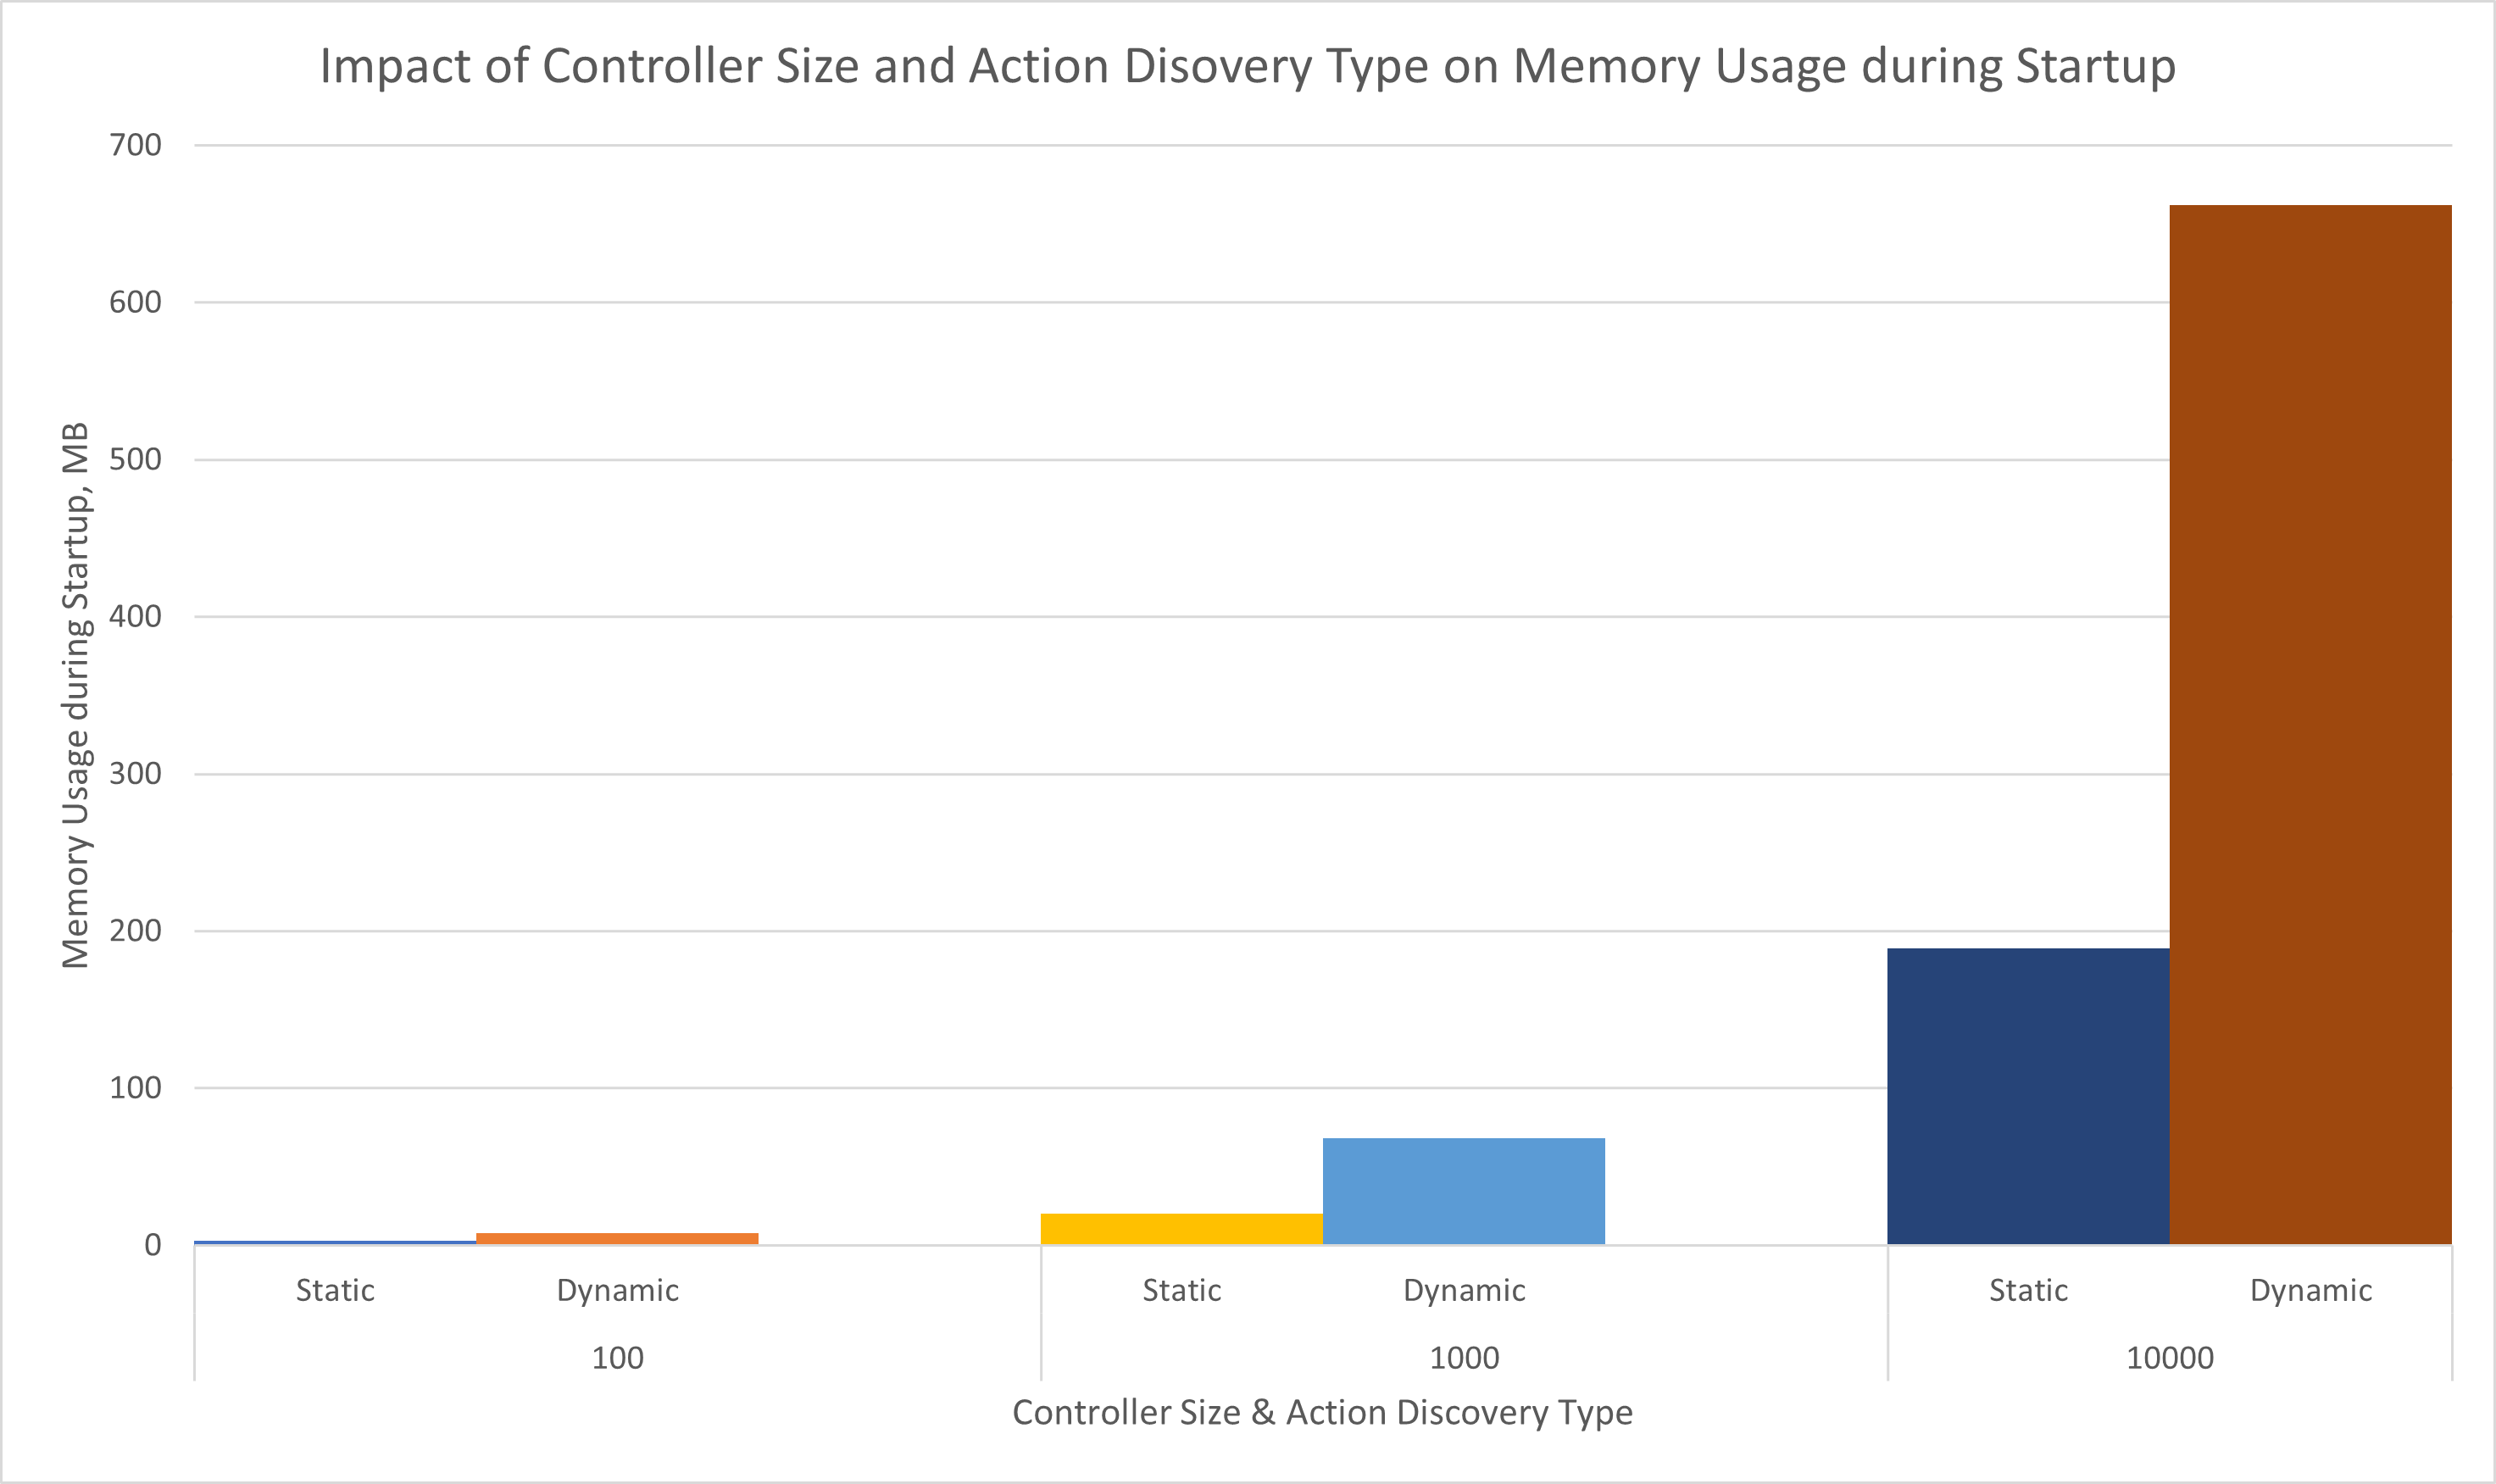
\includegraphics[width=0.8\textwidth]{graphics/Impact of Controller Size and Action Discovery Type on Memory Usage during Startup.png}
\caption{Impact of Controller Size and Action Discovery Type on Memory Usage during Startup}
\label{fig:memory-usage-results}
\end{figure}

A clear trend emerges from the data - the memory usage consistently increases in line with the number of controllers in an application. Specifically, the smallest application, consisting of 100 controllers, consumes 3 Megabytes (MB) of memory using static action discovery, while the dynamic approach uses more than double, at 8 MB.

Moving to the medium-sized application with 1,000 controllers, memory usage increases to 20 MB for the static method, while the dynamic counterpart demonstrates an even greater increase, reaching 68 MB.

Finally, the largest application of 10,000 controllers exhibits substantial memory usage: 189 MB for the static action discovery approach and a notably higher 662 MB for the dynamic method.
\chapter{Discussion}
\begin{itemize}
    \item Discuss the significance of the results, relating them to the initial objectives and existing literature. Explain the implications for using C\# source generators in similar scenarios.
    \item In-depth analysis of the study's findings
    \item Integration of the results with existing literature and theories
\end{itemize}

\section{Interpretation of Results}

\begin{itemize}
    \item Comprehensive analysis of the study's results
    \item Identification of key patterns and trends
\end{itemize}

\section{Comparison of Runtime Performance and Buildtime Duration}

\begin{itemize}
    \item Direct comparison of the performance metrics
    \item Evaluation of the trade-offs between runtime performance and buildtime duration
\end{itemize}

\section{Implications}

\begin{itemize}
    \item Discussion of the practical implications of the results for software developers
    \item Suggestions for improving software development practices using C\# source generators
\end{itemize}

\section{Limitations and Future Research}

\begin{itemize}
    \item Identification of limitations and potential biases in the study
    \item Suggestions for future research to address these limitations and expand upon the findings
\end{itemize}

\chapter{Conclusion}

The primary objective of this thesis was to investigate the impact of utilizing C\# source generators to convert reflective routing operations into static code in ASP.NET Core, specifically focusing on its effect on runtime performance, memory usage, and build duration. The research strived to establish the potential advantages and drawbacks of shifting from dynamic action discovery to static action discovery.

The key findings indicate that static action discovery can drastically reduce startup times and memory usage for ASP.NET Core applications. This change enhances the web server's overall performance, which benefits developers and businesses alike. Businesses may see reductions in operational costs due to improved server efficiency and resource usage. However, these gains come with the significant trade-off of longer build times, which currently presents a significant barrier to the widespread adoption of this approach.

In terms of practical implications, these findings can influence a developer's choice of action discovery techniques and potentially shape the design of future versions of ASP.NET Core or similar web development frameworks. While the extended build times are a limitation, they also highlight areas for further innovation and optimization within this approach.

Future research can explore several exciting avenues, building upon the findings of this study. One possibility is to expand static action discovery to include property generation. This enhancement could enable static action discovery in web technologies like Blazor or Razor. Such an expansion of scope could lead to broader usage and further improvements in application performance. Moreover, it would be valuable to investigate how static action discovery holds up in more complex applications, specifically those with a complicated startup phase. Additionally, it would be interesting to explore methods to determine constructor arguments or properties at compile-time more deterministically, potentially leading to more scenarios allowing the pre-generation of final values. With this study demonstrating the effective use of source generators in removing the need for runtime reflection, there is potential for significant performance improvements across the entire .NET ecosystem.

Despite the limitations identified, such as testing in a minimal setup, potential discrepancies between static and dynamic approaches, and unaccounted variables affecting the startup time, the study successfully demonstrates the potential of C# source generators to optimize ASP.NET Core applications' performance.

%\listoffigures

\listoftables
\printbibliography

\newpage

\begin{appendix}
\chapter*{Selbstständigkeitserklärung}
\todo[inline]{Rewrite in english}
Ich erkläre hiermit, dass ich diese Thesis selbständig verfasst 
und keine andern als die angegebenen Quellen benutzt habe. 
Alle Stellen, die wörtlich oder sinngemäss aus Quellen entnommen wurden, 
habe ich als solche kenntlich gemacht. Ich versichere zudem, dass ich bisher 
noch keine wissenschaftliche Arbeit mit gleichem oder ähnlichem Inhalt an der 
Fernfachhochschule Schweiz oder an einer anderen Hochschule eingereicht habe. 
Mir ist bekannt, dass andernfalls die Fernfachhochschule Schweiz zum Entzug 
des aufgrund dieser Thesis verliehenen Titels berechtigt ist.

\vspace{4cm}
\noindent
\hrule \ \\[-0.5ex]
Ort, Datum, Unterschrift
\end{appendix}

\end{document}